\chapter{多项式与矩阵方程}

% SOURCE_PDF_PAGE 179

\hypertarget{source-p179}{}
\phantomsection\addcontentsline{toc}{section}{3.1 竞赛要点与难点}
\phantomsection\addcontentsline{toc}{section}{3.2 范例解析与精讲}
全国大学生数学竞赛中，涉及多项式的考试内容主要包括:多项式整除、代数基本
\sourceblock{450.00}{images-full/p179-d000.png}
求解矩阵方程的题目(例如，第十四届全国初赛题及第七届全国决赛题).所谓矩阵方程
是指形如\allowbreak{}\raisebox{-3.12pt}{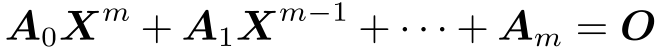
\includegraphics[width=186.45pt]{images-full/p179-i000.png}}\allowbreak{} 的方程，其中\allowbreak{}\raisebox{-2.76pt}{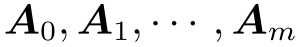
\includegraphics[width=85.31pt]{images-full/p179-i001.png}}\allowbreak{}是己知的\allowbreak{}\raisebox{-1.68pt}{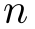
\includegraphics[width=9.60pt]{images-full/p179-i002.png}}\allowbreak{}
阶方阵，$x$ 是未知的\allowbreak{}\raisebox{-1.56pt}{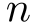
\includegraphics[width=10.17pt]{images-full/p179-i004.png}}\allowbreak{} 阶方阵.
\section*{3.1 竞赛要点与难点}
\par\noindent (1) 数域与一元多项式:一元多项式的基本性质; 多项式整除与带余除法;最大公因
式与最小公倍式; 互素、辗转相除法.
\par\noindent (2) 因式分解定理:不可约多项式的定义及性质，因式分解及唯一性定理;标准分解、
重因式及重根的定义，重因式存在的判定方法;多项式函数、余数定理、多项式的根及性
质等;代数基本定理、复系数与实系数多项式的因式分解.
\par\noindent (3) 有理系数多项式:本原多项式、Gauss (高斯)引理、有理系数多项式的因式分解、
Eisenstein (艾森斯坦)判别法、有理数域上多项式的有理根等.
\par\noindent (4) 多元多项式及对称多项式、Vieta 定理.
\section*{3.2 范例解析与精讲}
\sourceblock{190.97}{images-full/p179-d001.png}
\par\medskip\noindent\textbf{【例3.2.1 】设\allowbreak{}\raisebox{-1.68pt}{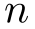
\includegraphics[width=9.60pt]{images-full/p179-i005.png}}\allowbreak{} 阶方阵$A$ 满足}
\sourceblock{110.74}{images-full/p179-d002.png}
其中$m$ 为正整数，证明\allowbreak{}\raisebox{-3.12pt}{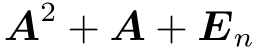
\includegraphics[width=72.88pt]{images-full/p179-i008.png}}\allowbreak{} 是可逆矩阵并求其逆.
\par\noindent\textbf{证明}\ 考察多项式
\sourceblock{223.74}{images-full/p179-d003.png}
则\allowbreak{}\raisebox{-3.00pt}{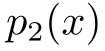
\includegraphics[width=29.38pt]{images-full/p179-i009.png}}\allowbreak{} 的根为\allowbreak{}\raisebox{-3.48pt}{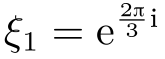
\includegraphics[width=46.33pt]{images-full/p179-i010.png}}\allowbreak{}和\allowbreak{}\raisebox{-3.48pt}{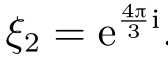
\includegraphics[width=47.17pt]{images-full/p179-i011.png}}\allowbreak{}


% SOURCE_PDF_PAGE 180

\hypertarget{source-p180}{}
将之代入\allowbreak{}\raisebox{-3.00pt}{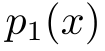
\includegraphics[width=29.38pt]{images-full/p180-i000.png}}\allowbreak{} 中，显见\allowbreak{}\raisebox{-3.00pt}{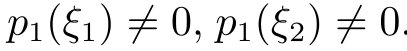
\includegraphics[width=114.79pt]{images-full/p180-i001.png}}\allowbreak{} 因而\allowbreak{}\raisebox{-3.00pt}{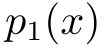
\includegraphics[width=29.38pt]{images-full/p180-i002.png}}\allowbreak{} 与\allowbreak{}\raisebox{-3.00pt}{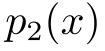
\includegraphics[width=29.38pt]{images-full/p180-i003.png}}\allowbreak{} 在复数域上无公
共根，进而\allowbreak{}\raisebox{-2.88pt}{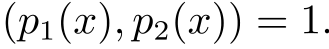
\includegraphics[width=92.57pt]{images-full/p180-i004.png}}\allowbreak{}.现在\allowbreak{}\raisebox{-3.00pt}{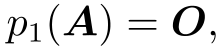
\includegraphics[width=60.73pt]{images-full/p180-i005.png}}\allowbreak{}，故有\allowbreak{}\raisebox{-3.00pt}{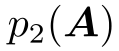
\includegraphics[width=33.33pt]{images-full/p180-i006.png}}\allowbreak{} 可逆. (事实上，设\allowbreak{}\raisebox{-2.76pt}{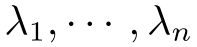
\includegraphics[width=55.37pt]{images-full/p180-i007.png}}\allowbreak{}
为$A$ 的\allowbreak{}\raisebox{-1.68pt}{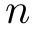
\includegraphics[width=10.17pt]{images-full/p180-i009.png}}\allowbreak{} 个特征值，则\allowbreak{}\raisebox{-3.24pt}{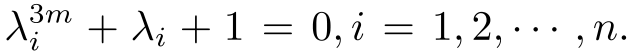
\includegraphics[width=176.79pt]{images-full/p180-i010.png}}\allowbreak{} 于是\allowbreak{}\raisebox{-3.24pt}{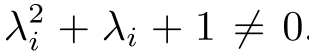
\includegraphics[width=87.14pt]{images-full/p180-i011.png}}\allowbreak{}故
\allowbreak{}\raisebox{-3.12pt}{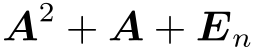
\includegraphics[width=72.88pt]{images-full/p180-i012.png}}\allowbreak{} 的\allowbreak{}\raisebox{-1.68pt}{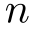
\includegraphics[width=9.60pt]{images-full/p180-i013.png}}\allowbreak{} 个特征值均不为0.)
为求出\allowbreak{}\raisebox{-3.12pt}{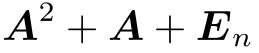
\includegraphics[width=72.88pt]{images-full/p180-i014.png}}\allowbreak{} 的逆，用带余除法，得
\sourceblock{319.22}{images-full/p180-d000.png}
注意到
\sourceblock{168.37}{images-full/p180-d001.png}
因此有
\sourceblock{390.41}{images-full/p180-d002.png}
故
\sourceblock{285.89}{images-full/p180-d003.png}
进而得
\sourceblock{444.09}{images-full/p180-d004.png}
\sourceblock{433.92}{images-full/p180-d005.png}
方面:一是，求矩阵的逆，如上例;二是，用于获取矩阵秩的有关等式与不等式;三是，获取
空间的分解;四是，几何性质的讨论等.其中空间的分解主要是指空间的直和分解.相关的
例子将在后续中给出.
\par\medskip\noindent\textbf{【例3.2.3 】在有理数域上，多项式\allowbreak{}\raisebox{-3.00pt}{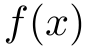
\includegraphics[width=24.86pt]{images-full/p181-i004.png}}\allowbreak{} 为}
\sourceblock{153.11}{images-full/p181-d000.png}
(其中\allowbreak{}\raisebox{-2.88pt}{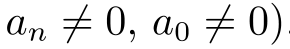
\includegraphics[width=81.73pt]{images-full/p181-i005.png}}\allowbreak{} 记\allowbreak{}\raisebox{-2.88pt}{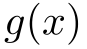
\includegraphics[width=24.29pt]{images-full/p181-i006.png}}\allowbreak{} 为
\sourceblock{377.98}{images-full/p181-d001.png}
于是
\sourceblock{78.53}{images-full/p181-d002.png}
若\allowbreak{}\raisebox{-3.00pt}{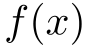
\includegraphics[width=25.42pt]{images-full/p181-i007.png}}\allowbreak{} 可约，不妨设\allowbreak{}\raisebox{-2.76pt}{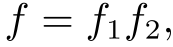
\includegraphics[width=48.57pt]{images-full/p181-i008.png}}\allowbreak{}其中\allowbreak{}\raisebox{-2.76pt}{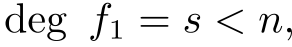
\includegraphics[width=82.23pt]{images-full/p181-i009.png}}\allowbreak{}，deg \allowbreak{}\raisebox{-2.76pt}{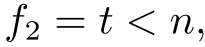
\includegraphics[width=57.54pt]{images-full/p181-i010.png}}\allowbreak{}则
\sourceblock{272.89}{images-full/p181-d003.png}
其中\allowbreak{}\raisebox{-3.00pt}{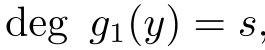
\includegraphics[width=74.49pt]{images-full/p181-i011.png}}\allowbreak{}, deg \allowbreak{}\raisebox{-3.00pt}{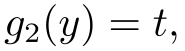
\includegraphics[width=51.98pt]{images-full/p181-i012.png}}\allowbreak{}故\allowbreak{}\raisebox{-3.00pt}{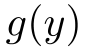
\includegraphics[width=24.29pt]{images-full/p181-i013.png}}\allowbreak{} 可约.
类似地，可证:若g(y) 可约，则f(x) 也可约.口
园也型五美于多项制制确定在证明
\par\medskip\noindent\textbf{【例3.2.5 】设\allowbreak{}\raisebox{-2.88pt}{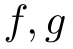
\includegraphics[width=20.34pt]{images-full/p182-i000.png}}\allowbreak{} 为两复系数多项式，$f$ 与$g$ 互素.证明:\allowbreak{}\raisebox{-3.24pt}{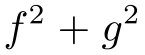
\includegraphics[width=40.68pt]{images-full/p182-i003.png}}\allowbreak{}的重根必为}
\allowbreak{}\raisebox{-3.24pt}{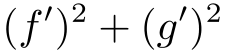
\includegraphics[width=64.41pt]{images-full/p182-i004.png}}\allowbreak{} 的根.
\par\noindent\textbf{证明}\ 设\allowbreak{}\raisebox{-1.68pt}{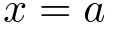
\includegraphics[width=31.64pt]{images-full/p182-i005.png}}\allowbreak{} 为\allowbreak{}\raisebox{-3.24pt}{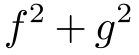
\includegraphics[width=38.98pt]{images-full/p182-i006.png}}\allowbreak{} 的重根.由\allowbreak{}\raisebox{-3.24pt}{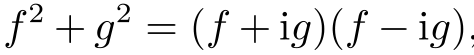
\includegraphics[width=133.42pt]{images-full/p182-i007.png}}\allowbreak{}，断言\allowbreak{}\raisebox{-1.68pt}{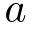
\includegraphics[width=9.04pt]{images-full/p182-i008.png}}\allowbreak{} 不是\allowbreak{}\raisebox{-2.88pt}{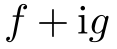
\includegraphics[width=32.77pt]{images-full/p182-i009.png}}\allowbreak{}
与\allowbreak{}\raisebox{-2.76pt}{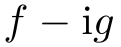
\includegraphics[width=33.90pt]{images-full/p182-i010.png}}\allowbreak{}的公共根.否则，有\allowbreak{}\raisebox{-3.00pt}{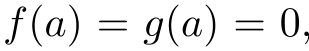
\includegraphics[width=87.00pt]{images-full/p182-i011.png}}\allowbreak{}，从而矛盾于$f$ 与$g$ 互素.这表明: \allowbreak{}\raisebox{-1.56pt}{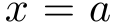
\includegraphics[width=32.77pt]{images-full/p182-i014.png}}\allowbreak{}
不是\allowbreak{}\raisebox{-2.76pt}{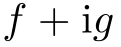
\includegraphics[width=33.90pt]{images-full/p182-i015.png}}\allowbreak{} 的重根就是\allowbreak{}\raisebox{-2.76pt}{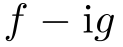
\includegraphics[width=34.46pt]{images-full/p182-i016.png}}\allowbreak{}的重根.不妨设\allowbreak{}\raisebox{-1.68pt}{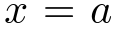
\includegraphics[width=33.33pt]{images-full/p182-i017.png}}\allowbreak{} 是\allowbreak{}\raisebox{-2.76pt}{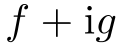
\includegraphics[width=34.46pt]{images-full/p182-i018.png}}\allowbreak{} 的重根.则有\allowbreak{}\raisebox{-1.68pt}{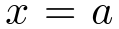
\includegraphics[width=33.33pt]{images-full/p182-i019.png}}\allowbreak{} 是
\allowbreak{}\raisebox{-3.12pt}{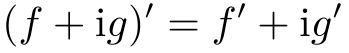
\includegraphics[width=98.31pt]{images-full/p182-i020.png}}\allowbreak{} 的根，进而: \allowbreak{}\raisebox{-3.36pt}{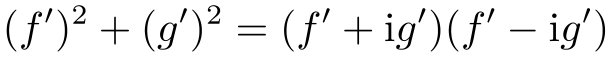
\includegraphics[width=172.89pt]{images-full/p182-i021.png}}\allowbreak{} 必以\allowbreak{}\raisebox{-1.68pt}{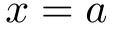
\includegraphics[width=31.64pt]{images-full/p182-i022.png}}\allowbreak{} 为根.口
\sourceblock{276.85}{images-full/p182-d000.png}
\sourceblock{163.28}{images-full/p182-d001.png}
\par\noindent\textbf{证明}\ :恰有\allowbreak{}\raisebox{-2.88pt}{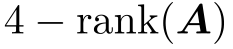
\includegraphics[width=65.54pt]{images-full/p182-i023.png}}\allowbreak{} 个4 次单位根是\allowbreak{}\raisebox{-2.88pt}{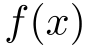
\includegraphics[width=24.86pt]{images-full/p182-i024.png}}\allowbreak{}的根(不计重数).
\sourceblock{267.81}{images-full/p182-d002.png}
则\allowbreak{}\raisebox{-3.48pt}{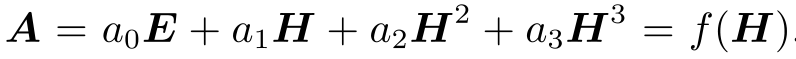
\includegraphics[width=224.61pt]{images-full/p182-i025.png}}\allowbreak{} 由于$H$ 的特征多项式\allowbreak{}\raisebox{-2.76pt}{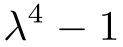
\includegraphics[width=34.46pt]{images-full/p182-i027.png}}\allowbreak{} 的4 个根
\allowbreak{}\raisebox{-2.76pt}{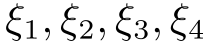
\includegraphics[width=58.76pt]{images-full/p182-i028.png}}\allowbreak{}各不相同，故$H$ 有\allowbreak{}\raisebox{-2.16pt}{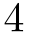
\includegraphics[width=8.47pt]{images-full/p182-i030.png}}\allowbreak{}个不同的特征值，进而
\sourceblock{142.38}{images-full/p182-d003.png}
\sourceblock{353.12}{images-full/p182-d004.png}
设\allowbreak{}\raisebox{-3.00pt}{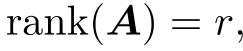
\includegraphics[width=68.45pt]{images-full/p182-i031.png}}\allowbreak{}则\allowbreak{}\raisebox{-3.00pt}{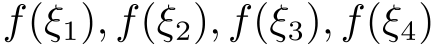
\includegraphics[width=123.73pt]{images-full/p182-i032.png}}\allowbreak{} 恰有\allowbreak{}\raisebox{-2.28pt}{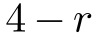
\includegraphics[width=27.68pt]{images-full/p182-i033.png}}\allowbreak{} 个为0，进而$f$ 恰有\allowbreak{}\raisebox{-2.28pt}{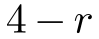
\includegraphics[width=27.68pt]{images-full/p182-i035.png}}\allowbreak{} 个4 次
单位根.口


% SOURCE_PDF_PAGE 183

\hypertarget{source-p183}{}
园也型回乡项制寺解脱用
\sourceblock{450.00}{images-full/p183-d000.png}
\par\noindent\textbf{证明}\ 考察\allowbreak{}\raisebox{-2.28pt}{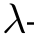
\includegraphics[width=9.44pt]{images-full/p183-i000.png}}\allowbreak{}矩阵
\sourceblock{164.41}{images-full/p183-d001.png}
为方便计，简记为
\sourceblock{450.00}{images-full/p183-d002.png}
\sourceblock{37.29}{images-full/p183-d003.png}
\sourceblock{450.00}{images-full/p183-d004.png}


% SOURCE_PDF_PAGE 184

\hypertarget{source-p184}{}
\sourceblock{450.00}{images-full/p184-d000.png}
【点评】此例也可看成是多项式的互素在证明矩阵秩等式中的应用.
\par\medskip\noindent\textbf{【例3.2.8 】设\allowbreak{}\raisebox{-3.00pt}{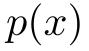
\includegraphics[width=24.86pt]{images-full/p184-i000.png}}\allowbreak{} 是实系数多项式，且对所有实数$z$均有\allowbreak{}\raisebox{-3.00pt}{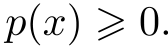
\includegraphics[width=46.94pt]{images-full/p184-i002.png}}\allowbreak{} 证明存在实}
\sourceblock{283.06}{images-full/p184-d001.png}
\par\noindent\textbf{证明}\ (1) 由于实系数多项式的根要么是实数，要么成共辄对出现. 因此可设\allowbreak{}\raisebox{-2.88pt}{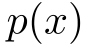
\includegraphics[width=24.86pt]{images-full/p184-i003.png}}\allowbreak{} 的
所有互不相同的实根为\allowbreak{}\raisebox{-3.00pt}{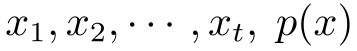
\includegraphics[width=100.57pt]{images-full/p184-i004.png}}\allowbreak{} 的具有正虚部的根为\allowbreak{}\raisebox{-2.04pt}{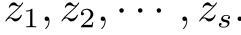
\includegraphics[width=67.84pt]{images-full/p184-i005.png}}\allowbreak{}·由条件，
\allowbreak{}\raisebox{-3.00pt}{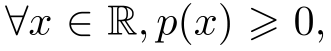
\includegraphics[width=93.22pt]{images-full/p184-i006.png}}\allowbreak{}，故有\allowbreak{}\raisebox{-2.04pt}{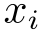
\includegraphics[width=12.43pt]{images-full/p184-i007.png}}\allowbreak{}的重数必为偶数\allowbreak{}\raisebox{-3.00pt}{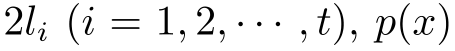
\includegraphics[width=128.25pt]{images-full/p184-i008.png}}\allowbreak{} 的首项系数\allowbreak{}\raisebox{-1.68pt}{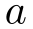
\includegraphics[width=9.04pt]{images-full/p184-i009.png}}\allowbreak{} 也必
大于O. 结果\allowbreak{}\raisebox{-3.00pt}{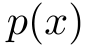
\includegraphics[width=24.86pt]{images-full/p184-i010.png}}\allowbreak{} 可写为
\sourceblock{226.00}{images-full/p184-d002.png}
\sourceblock{309.62}{images-full/p184-d003.png}
\allowbreak{}\raisebox{-3.12pt}{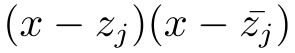
\includegraphics[width=83.05pt]{images-full/p184-i011.png}}\allowbreak{}可写为
\sourceblock{241.82}{images-full/p184-d004.png}
\sourceblock{257.64}{images-full/p184-d005.png}
故\allowbreak{}\raisebox{-2.88pt}{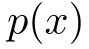
\includegraphics[width=24.86pt]{images-full/p184-i012.png}}\allowbreak{} 等于一些可表示为两个实系数多项式平方和的多项式的乘积.
\par\noindent (2) 断言:对两个实系数多项式的乘积，若它们中每一个都可表示为两个实系数多项
\sourceblock{450.00}{images-full/p184-d006.png}
故断言成立.
综上(1) ，(2)，故存在实系数多项式\allowbreak{}\raisebox{-3.00pt}{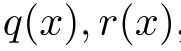
\includegraphics[width=50.86pt]{images-full/p184-i013.png}}\allowbreak{}，使得\allowbreak{}\raisebox{-3.24pt}{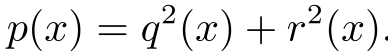
\includegraphics[width=109.55pt]{images-full/p184-i014.png}}\allowbreak{}口
\par\medskip\noindent\textbf{【例3.2.10 】设\allowbreak{}\raisebox{-2.04pt}{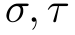
\includegraphics[width=20.90pt]{images-full/p185-i003.png}}\allowbreak{}为实$n$ 维向量空间$V$ 上的线性变换，\allowbreak{}\raisebox{-2.88pt}{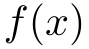
\includegraphics[width=24.86pt]{images-full/p185-i006.png}}\allowbreak{} 为\allowbreak{}\raisebox{-1.68pt}{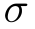
\includegraphics[width=9.60pt]{images-full/p185-i007.png}}\allowbreak{} 的特征多项}
式，证明: (1) \allowbreak{}\raisebox{-3.00pt}{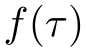
\includegraphics[width=24.29pt]{images-full/p185-i008.png}}\allowbreak{} 也是$V$ 上的线性变换; (2) \allowbreak{}\raisebox{-2.88pt}{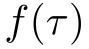
\includegraphics[width=24.86pt]{images-full/p185-i010.png}}\allowbreak{} 不是单射当且仅当\allowbreak{}\raisebox{-1.68pt}{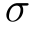
\includegraphics[width=9.60pt]{images-full/p185-i011.png}}\allowbreak{}与$T$有公共特
征值.
\par\noindent\textbf{证明}\ (1) 是显然的.
\par\noindent (2) 任取$V$ 的一组基\allowbreak{}\raisebox{-2.16pt}{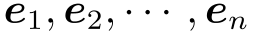
\includegraphics[width=71.22pt]{images-full/p185-i014.png}}\allowbreak{}，令
\sourceblock{403.97}{images-full/p185-d007.png}
则有\allowbreak{}\raisebox{-3.00pt}{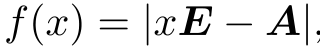
\includegraphics[width=89.91pt]{images-full/p185-i015.png}}\allowbreak{}，设\allowbreak{}\raisebox{-2.76pt}{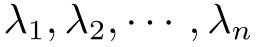
\includegraphics[width=72.32pt]{images-full/p185-i016.png}}\allowbreak{}为$A$ 的$n$ 个(复)特征值，\allowbreak{}\raisebox{-2.16pt}{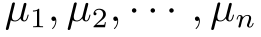
\includegraphics[width=73.45pt]{images-full/p185-i019.png}}\allowbreak{} 为$B$
的$n$个(复)特征值.于是
\sourceblock{100.57}{images-full/p185-d008.png}


% SOURCE_PDF_PAGE 186

\hypertarget{source-p186}{}
\sourceblock{239.56}{images-full/p186-d000.png}
所以\allowbreak{}\raisebox{-3.00pt}{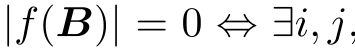
\includegraphics[width=99.80pt]{images-full/p186-i000.png}}\allowbreak{}，S.t. \allowbreak{}\raisebox{-3.00pt}{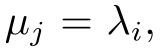
\includegraphics[width=45.11pt]{images-full/p186-i001.png}}\allowbreak{}，即\allowbreak{}\raisebox{-3.00pt}{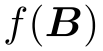
\includegraphics[width=28.81pt]{images-full/p186-i002.png}}\allowbreak{} 为奇异矩阵等价于$A$ 与$B$ 有公共特征
根.注意到\allowbreak{}\raisebox{-3.00pt}{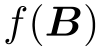
\includegraphics[width=28.81pt]{images-full/p186-i005.png}}\allowbreak{} 为\allowbreak{}\raisebox{-3.00pt}{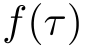
\includegraphics[width=24.29pt]{images-full/p186-i006.png}}\allowbreak{} 在基\allowbreak{}\raisebox{-2.16pt}{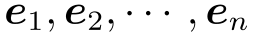
\includegraphics[width=71.75pt]{images-full/p186-i007.png}}\allowbreak{} 下的表示阵，因此有\allowbreak{}\raisebox{-3.00pt}{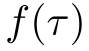
\includegraphics[width=24.86pt]{images-full/p186-i008.png}}\allowbreak{} 为非同构变换等
价于\allowbreak{}\raisebox{-1.68pt}{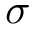
\includegraphics[width=9.60pt]{images-full/p186-i009.png}}\allowbreak{}与$T$有公共特征值.
最后，有限维空间上的线性变换，它为同构当且仅当它为单射，也等价于它为满射.故
得
\par \allowbreak{}\raisebox{-3.00pt}{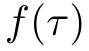
\includegraphics[width=24.86pt]{images-full/p186-i011.png}}\allowbreak{} 不是单射\allowbreak{}\raisebox{-1.92pt}{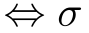
\includegraphics[width=24.86pt]{images-full/p186-i012.png}}\allowbreak{} 与$T$ 有公共特征值.口
国也型λ据眸方程
\par\medskip\noindent\textbf{【例3.2.13 】设\allowbreak{}\raisebox{-3.24pt}{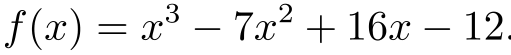
\includegraphics[width=144.26pt]{images-full/p187-i000.png}}\allowbreak{} 试求\allowbreak{}\raisebox{-3.00pt}{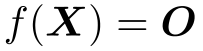
\includegraphics[width=57.06pt]{images-full/p187-i001.png}}\allowbreak{} 的所有3 阶实方阵}
解\allowbreak{}\raisebox{-2.28pt}{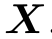
\includegraphics[width=14.27pt]{images-full/p187-i002.png}}\allowbreak{}
解注意到:$X$ 是\allowbreak{}\raisebox{-3.00pt}{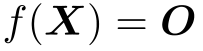
\includegraphics[width=56.99pt]{images-full/p187-i004.png}}\allowbreak{} 的解\allowbreak{}\raisebox{-3.00pt}{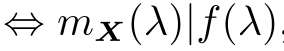
\includegraphics[width=80.08pt]{images-full/p187-i005.png}}\allowbreak{}，这里\allowbreak{}\raisebox{-3.00pt}{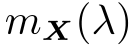
\includegraphics[width=38.42pt]{images-full/p187-i006.png}}\allowbreak{})表示$X$ 的最小多
项式.由\allowbreak{}\raisebox{-3.24pt}{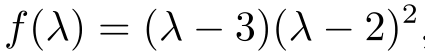
\includegraphics[width=119.73pt]{images-full/p187-i008.png}}\allowbreak{}，可知该矩阵方程的所有3 阶实方阵解$X$ 可能的初等因
子分别是
\sourceblock{338.43}{images-full/p187-d002.png}
\allowbreak{}\raisebox{-3.00pt}{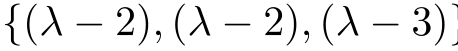
\includegraphics[width=128.99pt]{images-full/p187-i010.png}}\allowbreak{}\},\allowbreak{}\raisebox{-3.00pt}{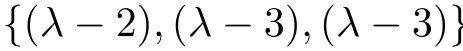
\includegraphics[width=130.34pt]{images-full/p187-i011.png}}\allowbreak{} ，\allowbreak{}\raisebox{-3.00pt}{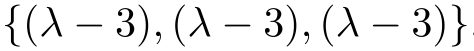
\includegraphics[width=133.82pt]{images-full/p187-i012.png}}\allowbreak{}.
\sourceblock{450.00}{images-full/p187-d003.png}


% SOURCE_PDF_PAGE 188

\hypertarget{source-p188}{}
\phantomsection\addcontentsline{toc}{section}{3.3 真题选讲与点评}
\par\medskip\noindent\textbf{【例3.2.14 】设\allowbreak{}\raisebox{-2.76pt}{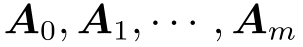
\includegraphics[width=85.31pt]{images-full/p188-i000.png}}\allowbreak{} 为\allowbreak{}\raisebox{-1.68pt}{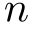
\includegraphics[width=10.17pt]{images-full/p188-i001.png}}\allowbreak{} 阶己知复方阵，\allowbreak{}\raisebox{-3.12pt}{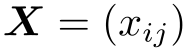
\includegraphics[width=53.67pt]{images-full/p188-i002.png}}\allowbreak{} 是$n$ 阶未知方阵}
\sourceblock{375.72}{images-full/p188-d000.png}
\sourceblock{222.04}{images-full/p188-d001.png}
\par\noindent\textbf{证明}\ : \allowbreak{}\raisebox{-3.00pt}{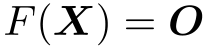
\includegraphics[width=58.76pt]{images-full/p188-i004.png}}\allowbreak{} 的解集必是\allowbreak{}\raisebox{-3.00pt}{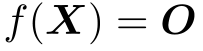
\includegraphics[width=57.06pt]{images-full/p188-i005.png}}\allowbreak{} 的解集的子集.
\par\noindent\textbf{证明}\ 对任意方阵$A$，有
\sourceblock{445.78}{images-full/p188-d002.png}
若\allowbreak{}\raisebox{-3.00pt}{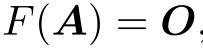
\includegraphics[width=57.03pt]{images-full/p188-i007.png}}\allowbreak{}，则\allowbreak{}\raisebox{-3.00pt}{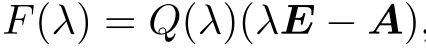
\includegraphics[width=119.92pt]{images-full/p188-i008.png}}\allowbreak{}，从而
\sourceblock{310.18}{images-full/p188-d003.png}
其中\allowbreak{}\raisebox{-3.00pt}{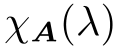
\includegraphics[width=33.90pt]{images-full/p188-i009.png}}\allowbreak{} 为$A$ 的特征多项式.由Hamilton (哈密顿)定理知，\allowbreak{}\raisebox{-3.00pt}{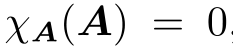
\includegraphics[width=65.38pt]{images-full/p188-i011.png}}\allowbreak{}，故有
\sourceblock{450.00}{images-full/p188-d004.png}
\par 但.3真题选讲与点评)
\par\medskip\noindent\textbf{【例3.3.1 】(第十一届全国初赛题)设$A$ 为\allowbreak{}\raisebox{-1.68pt}{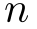
\includegraphics[width=10.17pt]{images-full/p188-i013.png}}\allowbreak{} 阶复方阵，\allowbreak{}\raisebox{-3.00pt}{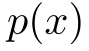
\includegraphics[width=24.86pt]{images-full/p188-i014.png}}\allowbreak{} 为\allowbreak{}\raisebox{-2.76pt}{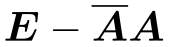
\includegraphics[width=48.02pt]{images-full/p188-i015.png}}\allowbreak{} 的特征}
多项式，其中\allowbreak{}\raisebox{-2.64pt}{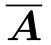
\includegraphics[width=14.12pt]{images-full/p188-i016.png}}\allowbreak{}表示$A$ 的共辄矩阵证明: \allowbreak{}\raisebox{-3.00pt}{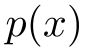
\includegraphics[width=24.29pt]{images-full/p188-i018.png}}\allowbreak{} 必为实系数多项式.
\par\noindent\textbf{证明}\ 设\allowbreak{}\raisebox{-2.64pt}{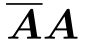
\includegraphics[width=23.73pt]{images-full/p188-i019.png}}\allowbreak{} 的Jordan 分解为
\sourceblock{276.28}{images-full/p188-d005.png}
其中\allowbreak{}\raisebox{-1.56pt}{
\includegraphics[width=7.91pt]{images-full/p188-i020.png}}\allowbreak{}为1 或\allowbreak{}\raisebox{-2.64pt}{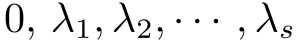
\includegraphics[width=84.75pt]{images-full/p188-i021.png}}\allowbreak{}为实特征值，\allowbreak{}\raisebox{-2.16pt}{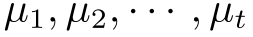
\includegraphics[width=71.19pt]{images-full/p188-i022.png}}\allowbreak{} 为非实的特征值.


% SOURCE_PDF_PAGE 189

\hypertarget{source-p189}{}
\sourceblock{450.00}{images-full/p189-d000.png}
\sourceblock{149.16}{images-full/p189-d001.png}
\sourceblock{285.32}{images-full/p189-d002.png}
注意到\allowbreak{}\raisebox{-2.76pt}{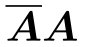
\includegraphics[width=23.73pt]{images-full/p189-i000.png}}\allowbreak{} 与\allowbreak{}\raisebox{-2.76pt}{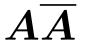
\includegraphics[width=23.73pt]{images-full/p189-i001.png}}\allowbreak{}有相同的特征多项式，因此数组\allowbreak{}\raisebox{-2.16pt}{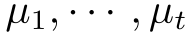
\includegraphics[width=53.67pt]{images-full/p189-i002.png}}\allowbreak{}与数组\allowbreak{}\raisebox{-2.52pt}{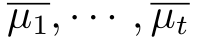
\includegraphics[width=55.37pt]{images-full/p189-i003.png}}\allowbreak{}是同一
数组.不妨设\allowbreak{}\raisebox{-2.64pt}{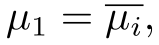
\includegraphics[width=44.63pt]{images-full/p189-i004.png}}\allowbreak{}，于是数组\allowbreak{}\raisebox{-2.16pt}{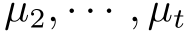
\includegraphics[width=53.67pt]{images-full/p189-i005.png}}\allowbreak{}与数组\allowbreak{}\raisebox{-2.64pt}{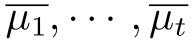
\includegraphics[width=54.80pt]{images-full/p189-i006.png}}\allowbreak{}挖掉了\allowbreak{}\raisebox{-2.64pt}{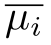
\includegraphics[width=14.12pt]{images-full/p189-i007.png}}\allowbreak{}后剩下的数组仍
然为同一数组.重复前述过程知，\allowbreak{}\raisebox{-2.64pt}{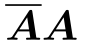
\includegraphics[width=23.73pt]{images-full/p189-i008.png}}\allowbreak{} 的非实特征值共辄成对出现，进而\allowbreak{}\raisebox{-2.64pt}{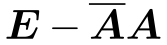
\includegraphics[width=46.89pt]{images-full/p189-i009.png}}\allowbreak{} 的非实
特征值也共辄成对出现.至此立即知\allowbreak{}\raisebox{-3.00pt}{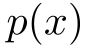
\includegraphics[width=24.86pt]{images-full/p189-i010.png}}\allowbreak{} 必为实系数多项式.口
\par\medskip\noindent\textbf{【例3.3.2 】(第十二届全国初赛题)称非常值一元$n$次多项式(含合并同类项后)的}
\allowbreak{}\raisebox{-2.28pt}{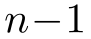
\includegraphics[width=25.42pt]{images-full/p189-i012.png}}\allowbreak{}次项(可能为0) 为第二项.求所有2020 次复系数首一多项式\allowbreak{}\raisebox{-2.88pt}{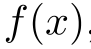
\includegraphics[width=25.38pt]{images-full/p189-i013.png}}\allowbreak{}，满足对\allowbreak{}\raisebox{-2.88pt}{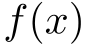
\includegraphics[width=24.86pt]{images-full/p189-i014.png}}\allowbreak{} 的每
个复根\allowbreak{}\raisebox{-2.16pt}{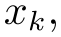
\includegraphics[width=16.72pt]{images-full/p189-i015.png}}\allowbreak{}都有非常值复系数首一多项式\allowbreak{}\raisebox{-3.00pt}{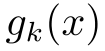
\includegraphics[width=29.38pt]{images-full/p189-i016.png}}\allowbreak{} 和\allowbreak{}\raisebox{-3.00pt}{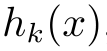
\includegraphics[width=30.00pt]{images-full/p189-i017.png}}\allowbreak{}，使得\allowbreak{}\raisebox{-3.00pt}{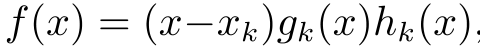
\includegraphics[width=135.26pt]{images-full/p189-i018.png}}\allowbreak{},
且\allowbreak{}\raisebox{-3.00pt}{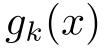
\includegraphics[width=29.38pt]{images-full/p189-i019.png}}\allowbreak{}与\allowbreak{}\raisebox{-3.00pt}{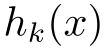
\includegraphics[width=29.94pt]{images-full/p189-i020.png}}\allowbreak{} 的第二项系数相等.
\par\noindent\textbf{证明}\ 显然，\allowbreak{}\raisebox{-3.36pt}{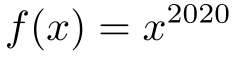
\includegraphics[width=66.10pt]{images-full/p189-i021.png}}\allowbreak{}满足题意.
下证这是满足题意的唯一解.设\allowbreak{}\raisebox{-3.00pt}{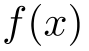
\includegraphics[width=24.86pt]{images-full/p189-i022.png}}\allowbreak{} 的2020 个复根为\allowbreak{}\raisebox{-2.04pt}{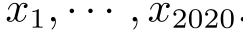
\includegraphics[width=68.34pt]{images-full/p189-i023.png}}\allowbreak{} 对每个\allowbreak{}\raisebox{-2.88pt}{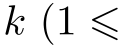
\includegraphics[width=35.03pt]{images-full/p189-i024.png}}\allowbreak{}
\allowbreak{}\raisebox{-3.00pt}{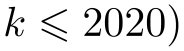
\includegraphics[width=51.76pt]{images-full/p189-i025.png}}\allowbreak{}，由题设知可设\allowbreak{}\raisebox{-3.00pt}{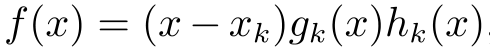
\includegraphics[width=137.97pt]{images-full/p189-i026.png}}\allowbreak{}，其中，\allowbreak{}\raisebox{-3.00pt}{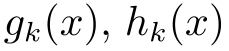
\includegraphics[width=64.41pt]{images-full/p189-i027.png}}\allowbreak{} 分别为\allowbreak{}\raisebox{-2.04pt}{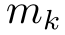
\includegraphics[width=18.08pt]{images-full/p189-i028.png}}\allowbreak{} 次和
\allowbreak{}\raisebox{-2.04pt}{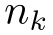
\includegraphics[width=14.69pt]{images-full/p189-i029.png}}\allowbreak{} 次非常值首一多项式，第二项系数均为\allowbreak{}\raisebox{-2.04pt}{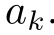
\includegraphics[width=14.92pt]{images-full/p189-i030.png}}\allowbreak{} 现设\allowbreak{}\raisebox{-3.00pt}{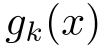
\includegraphics[width=29.38pt]{images-full/p189-i031.png}}\allowbreak{} 的所有复根为\allowbreak{}\raisebox{-2.28pt}{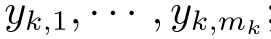
\includegraphics[width=76.00pt]{images-full/p189-i032.png}}\allowbreak{}
\allowbreak{}\raisebox{-3.00pt}{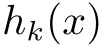
\includegraphics[width=29.94pt]{images-full/p189-i033.png}}\allowbreak{} 的所有复根为句\allowbreak{}\raisebox{-2.28pt}{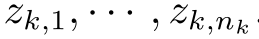
\includegraphics[width=73.01pt]{images-full/p189-i034.png}}\allowbreak{} 这些根恰为所有\allowbreak{}\raisebox{-3.12pt}{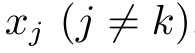
\includegraphics[width=54.80pt]{images-full/p189-i035.png}}\allowbreak{} 由Vieta 定理，
\sourceblock{289.84}{images-full/p189-d003.png}
\sourceblock{450.00}{images-full/p189-d004.png}
$A$ 为2020 阶方阵，主对角线上元素皆为\allowbreak{}\raisebox{-2.64pt}{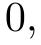
\includegraphics[width=11.30pt]{images-full/p189-i037.png}}\allowbreak{}，主对角线外元素皆为1 或\allowbreak{}\raisebox{-2.16pt}{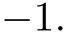
\includegraphics[width=19.77pt]{images-full/p189-i038.png}}\allowbreak{}令$B$ 为2020 阶
方阵，主对角线上元素皆为0，主对角线外元素全为1 ，则有$B$ 的行列式\allowbreak{}\raisebox{-2.28pt}{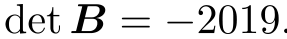
\includegraphics[width=80.78pt]{images-full/p189-i041.png}}\allowbreak{}.
由行列式定义，\allowbreak{}\raisebox{-2.40pt}{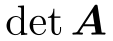
\includegraphics[width=31.64pt]{images-full/p189-i042.png}}\allowbreak{} 与\allowbreak{}\raisebox{-2.28pt}{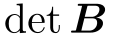
\includegraphics[width=31.64pt]{images-full/p189-i043.png}}\allowbreak{} 的奇偶性相同，故\allowbreak{}\raisebox{-2.88pt}{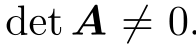
\includegraphics[width=55.22pt]{images-full/p189-i044.png}}\allowbreak{} 从而上述齐次线性方程组
只有零解，即\allowbreak{}\raisebox{-2.64pt}{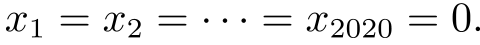
\includegraphics[width=135.38pt]{images-full/p189-i045.png}}\allowbreak{} 这就证明了
\sourceblock{263.85}{images-full/p189-d005.png}


% SOURCE_PDF_PAGE 190

\hypertarget{source-p190}{}
【点词唱此题是一道关于多项式的试题.它可看成是Vieta 定理的应用.由\allowbreak{}\raisebox{-2.40pt}{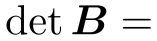
\includegraphics[width=44.07pt]{images-full/p190-i000.png}}\allowbreak{}
-2019 推出\allowbreak{}\raisebox{-2.76pt}{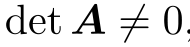
\includegraphics[width=53.31pt]{images-full/p190-i001.png}}\allowbreak{}，实际上，它也可由下列等式而得:
\sourceblock{201.70}{images-full/p190-d000.png}
其中\allowbreak{}\raisebox{-3.36pt}{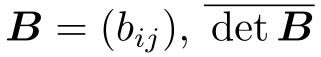
\includegraphics[width=90.40pt]{images-full/p190-i002.png}}\allowbreak{} 表示\allowbreak{}\raisebox{-2.40pt}{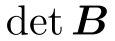
\includegraphics[width=32.20pt]{images-full/p190-i003.png}}\allowbreak{} 关于模2 取余，\allowbreak{}\raisebox{-3.36pt}{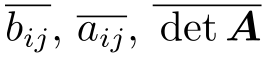
\includegraphics[width=75.71pt]{images-full/p190-i004.png}}\allowbreak{}类似.
\par\medskip\noindent\textbf{【例3.3.3】(第十二届全国初赛题)设$A$ 为$n$ 阶复方阵，\allowbreak{}\raisebox{-3.00pt}{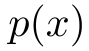
\includegraphics[width=24.86pt]{images-full/p190-i007.png}}\allowbreak{} 为$A$ 的特征多项式.}
又设\allowbreak{}\raisebox{-3.00pt}{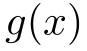
\includegraphics[width=24.29pt]{images-full/p190-i009.png}}\allowbreak{} 为$m$ 次复系数多项式，\allowbreak{}\raisebox{-2.52pt}{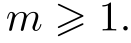
\includegraphics[width=36.77pt]{images-full/p190-i011.png}}\allowbreak{}.证明: \allowbreak{}\raisebox{-3.00pt}{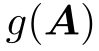
\includegraphics[width=27.68pt]{images-full/p190-i012.png}}\allowbreak{} 可逆当且仅当\allowbreak{}\raisebox{-3.00pt}{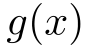
\includegraphics[width=24.29pt]{images-full/p190-i013.png}}\allowbreak{} 与\allowbreak{}\raisebox{-3.00pt}{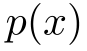
\includegraphics[width=24.29pt]{images-full/p190-i014.png}}\allowbreak{} 互素.
\par\noindent\textbf{证明}\ 取$A$ 的Jordan 分解
\sourceblock{163.85}{images-full/p190-d001.png}
\sourceblock{296.62}{images-full/p190-d002.png}
为Jordan 块于是
\sourceblock{385.89}{images-full/p190-d003.png}
充分性\allowbreak{}\raisebox{-2.88pt}{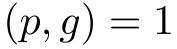
\includegraphics[width=49.72pt]{images-full/p190-i016.png}}\allowbreak{}时，$g$ 与$p$ 没有公共根.故\allowbreak{}\raisebox{-3.00pt}{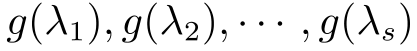
\includegraphics[width=117.52pt]{images-full/p190-i019.png}}\allowbreak{} 皆不为\allowbreak{}\raisebox{-2.28pt}{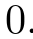
\includegraphics[width=8.95pt]{images-full/p190-i020.png}}\allowbreak{} 显然
此时有\allowbreak{}\raisebox{-2.88pt}{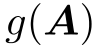
\includegraphics[width=27.68pt]{images-full/p190-i021.png}}\allowbreak{} 可逆
必要性由\allowbreak{}\raisebox{-3.00pt}{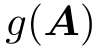
\includegraphics[width=27.68pt]{images-full/p190-i022.png}}\allowbreak{} 可逆知，\allowbreak{}\raisebox{-3.00pt}{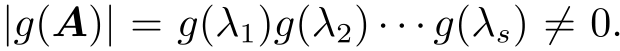
\includegraphics[width=174.93pt]{images-full/p190-i023.png}}\allowbreak{} 因此机\allowbreak{}\raisebox{-2.76pt}{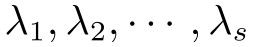
\includegraphics[width=71.19pt]{images-full/p190-i024.png}}\allowbreak{} 均
不是\allowbreak{}\raisebox{-3.00pt}{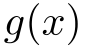
\includegraphics[width=24.29pt]{images-full/p190-i025.png}}\allowbreak{} 的根.注意到，\allowbreak{}\raisebox{-2.76pt}{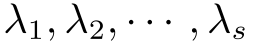
\includegraphics[width=71.19pt]{images-full/p190-i026.png}}\allowbreak{}遍历\allowbreak{}\raisebox{-3.00pt}{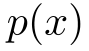
\includegraphics[width=24.86pt]{images-full/p190-i027.png}}\allowbreak{} 的所有根，从而$g$ 与$p$ 没有公共根，
\allowbreak{}\raisebox{-3.00pt}{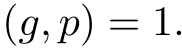
\includegraphics[width=51.14pt]{images-full/p190-i030.png}}\allowbreak{}1.口
\sourceblock{450.00}{images-full/p190-d004.png}
\allowbreak{}\raisebox{-3.00pt}{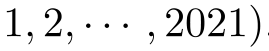
\includegraphics[width=75.59pt]{images-full/p190-i031.png}}\allowbreak{} 若\allowbreak{}\raisebox{-2.04pt}{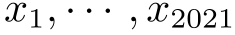
\includegraphics[width=66.10pt]{images-full/p190-i032.png}}\allowbreak{} 均是实数，则由Cauchy 不等式有
\sourceblock{216.39}{images-full/p190-d005.png}


% SOURCE_PDF_PAGE 191

\hypertarget{source-p191}{}
\sourceblock{342.39}{images-full/p191-d000.png}
由此得
\sourceblock{328.26}{images-full/p191-d001.png}
\sourceblock{350.86}{images-full/p191-d002.png}
的根，因此又由Vieta 定理得
\sourceblock{216.96}{images-full/p191-d003.png}
\sourceblock{368.94}{images-full/p191-d004.png}
困为对任意的\allowbreak{}\raisebox{-2.64pt}{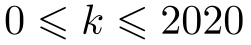
\includegraphics[width=70.62pt]{images-full/p191-i000.png}}\allowbreak{} 有\allowbreak{}\raisebox{-3.00pt}{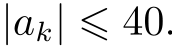
\includegraphics[width=48.30pt]{images-full/p191-i001.png}}\allowbreak{} 又\allowbreak{}\raisebox{-2.04pt}{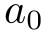
\includegraphics[width=13.56pt]{images-full/p191-i002.png}}\allowbreak{}为非0 整数，故\allowbreak{}\raisebox{-3.00pt}{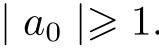
\includegraphics[width=44.74pt]{images-full/p191-i003.png}}\allowbreak{}.结果
\sourceblock{255.38}{images-full/p191-d005.png}
矛盾.口
【点评】此题考察的是Vieta 定理的应用.解题过程中涉及Schwarz 不等式或
\sourceblock{401.71}{images-full/p191-d006.png}
\sourceblock{181.36}{images-full/p191-d007.png}


% SOURCE_PDF_PAGE 192

\hypertarget{source-p192}{}
此不等式又称为离散的Hölder (霍尔德)不等式.连续的Hölder 不等式则是针对积分估
计，其内容则为:设\allowbreak{}\raisebox{-2.16pt}{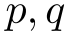
\includegraphics[width=20.34pt]{images-full/p192-i000.png}}\allowbreak{} 同上，\allowbreak{}\raisebox{-3.00pt}{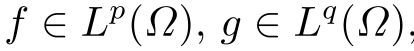
\includegraphics[width=116.57pt]{images-full/p192-i001.png}}\allowbreak{}，则有
\sourceblock{260.46}{images-full/p192-d000.png}
\par\medskip\noindent\textbf{【例3.3.5 \allowbreak{}\raisebox{-3.12pt}{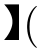
\includegraphics[width=11.75pt]{images-full/p192-i002.png}}\allowbreak{}(第十四届全国初赛题)设\allowbreak{}\raisebox{-2.64pt}{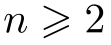
\includegraphics[width=31.07pt]{images-full/p192-i003.png}}\allowbreak{} 为正整数，证明多项式\allowbreak{}\raisebox{-3.00pt}{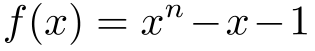
\includegraphics[width=88.70pt]{images-full/p192-i004.png}}\allowbreak{}}
在有理数域$Q$ 上不可约.
\par\noindent\textbf{证明}\ 对任意多项式\allowbreak{}\raisebox{-3.24pt}{\includegraphics[width=219.60pt]{images-full/p192-i006.png}}\allowbreak{}，用\allowbreak{}\raisebox{-3.48pt}{\includegraphics[width=27.12pt]{images-full/p192-i007.png}}\allowbreak{}表示\allowbreak{}\raisebox{-2.88pt}{\includegraphics[width=27.12pt]{images-full/p192-i008.png}}\allowbreak{}
的互反多项式，即
\sourceblock{302.27}{images-full/p192-d001.png}
\sourceblock{450.00}{images-full/p192-d002.png}
G(x)H(x) 是互反多项式G(x) 和H(x) 的乘积.
下面证明\allowbreak{}\raisebox{-3.00pt}{\includegraphics[width=94.92pt]{images-full/p192-i009.png}}\allowbreak{}在有理数域Q 上不可约.若\allowbreak{}\raisebox{-2.64pt}{\includegraphics[width=33.38pt]{images-full/p192-i010.png}}\allowbreak{}则结论显然成立.
下面设\allowbreak{}\raisebox{-2.52pt}{\includegraphics[width=37.70pt]{images-full/p192-i011.png}}\allowbreak{}若\allowbreak{}\raisebox{-3.00pt}{\includegraphics[width=24.86pt]{images-full/p192-i012.png}}\allowbreak{} 在$Q$ 上可约，由于\allowbreak{}\raisebox{-3.00pt}{\includegraphics[width=24.86pt]{images-full/p192-i014.png}}\allowbreak{} 本原，所以存在整系数多项式
\allowbreak{}\raisebox{-3.00pt}{\includegraphics[width=88.14pt]{images-full/p192-i015.png}}\allowbreak{}使得\allowbreak{}\raisebox{-3.00pt}{\includegraphics[width=85.88pt]{images-full/p192-i016.png}}\allowbreak{} 且\allowbreak{}\raisebox{-3.00pt}{\includegraphics[width=110.31pt]{images-full/p192-i017.png}}\allowbreak{} 这时\allowbreak{}\raisebox{-3.00pt}{\includegraphics[width=87.66pt]{images-full/p192-i018.png}}\allowbreak{}
进一步地，由于\allowbreak{}\raisebox{-3.00pt}{\includegraphics[width=24.86pt]{images-full/p192-i019.png}}\allowbreak{} 的首项系数为1，常数项为\allowbreak{}\raisebox{-2.52pt}{\includegraphics[width=17.36pt]{images-full/p192-i020.png}}\allowbreak{}，我们可以假设\allowbreak{}\raisebox{-3.00pt}{\includegraphics[width=24.29pt]{images-full/p192-i021.png}}\allowbreak{} 和\allowbreak{}\raisebox{-3.00pt}{\includegraphics[width=24.29pt]{images-full/p192-i022.png}}\allowbreak{} 的首项
系数均为1，而它们的常数项只能是土1.令\allowbreak{}\raisebox{-3.60pt}{\includegraphics[width=127.12pt]{images-full/p192-i023.png}}\allowbreak{}，由于\allowbreak{}\raisebox{-3.60pt}{\includegraphics[width=57.06pt]{images-full/p192-i024.png}}\allowbreak{}
\allowbreak{}\raisebox{-3.00pt}{\includegraphics[width=87.29pt]{images-full/p192-i025.png}}\allowbreak{}我们有\allowbreak{}\raisebox{-3.00pt}{\includegraphics[width=68.04pt]{images-full/p192-i026.png}}\allowbreak{}且
\sourceblock{337.30}{images-full/p192-d003.png}
显然\allowbreak{}\raisebox{-3.60pt}{\includegraphics[width=125.43pt]{images-full/p192-i027.png}}\allowbreak{}，所以
\sourceblock{289.84}{images-full/p192-d004.png}
记\allowbreak{}\raisebox{-3.24pt}{\includegraphics[width=213.02pt]{images-full/p192-i028.png}}\allowbreak{}，则显然有\allowbreak{}\raisebox{-2.64pt}{\includegraphics[width=60.68pt]{images-full/p192-i029.png}}\allowbreak{}.比较(3.3.1) 式两端
f 的系数得到
\sourceblock{450.00}{images-full/p192-d005.png}
由此得到
\sourceblock{394.37}{images-full/p192-d006.png}
下面看(3.3.1) 式中次数\allowbreak{}\raisebox{-1.92pt}{\includegraphics[width=22.03pt]{images-full/p192-i030.png}}\allowbreak{} 的各项系数，常数项\allowbreak{}\raisebox{-2.64pt}{\includegraphics[width=55.99pt]{images-full/p192-i031.png}}\allowbreak{}，由此得到\allowbreak{}\raisebox{-2.64pt}{\includegraphics[width=52.54pt]{images-full/p192-i032.png}}\allowbreak{} 又由
\allowbreak{}\raisebox{-2.52pt}{\includegraphics[width=32.77pt]{images-full/p192-i033.png}}\allowbreak{} 有\allowbreak{}\raisebox{-2.64pt}{\includegraphics[width=78.32pt]{images-full/p192-i034.png}}\allowbreak{}，所以\allowbreak{}\raisebox{-2.88pt}{\includegraphics[width=50.24pt]{images-full/p192-i035.png}}\allowbreak{} 若\allowbreak{}\raisebox{-2.64pt}{\includegraphics[width=52.54pt]{images-full/p192-i036.png}}\allowbreak{}，则有\allowbreak{}\raisebox{-2.16pt}{\includegraphics[width=28.81pt]{images-full/p192-i037.png}}\allowbreak{} 且\allowbreak{}\raisebox{-2.76pt}{\includegraphics[width=77.11pt]{images-full/p192-i038.png}}\allowbreak{}这


% SOURCE_PDF_PAGE 193

\hypertarget{source-p193}{}
\sourceblock{450.00}{images-full/p193-d000.png}
若\allowbreak{}\raisebox{-3.00pt}{\includegraphics[width=75.06pt]{images-full/p193-i000.png}}\allowbreak{}，则有\allowbreak{}\raisebox{-3.60pt}{\includegraphics[width=74.84pt]{images-full/p193-i001.png}}\allowbreak{} 故\allowbreak{}\raisebox{-3.00pt}{\includegraphics[width=24.86pt]{images-full/p193-i002.png}}\allowbreak{} 的任一复根就是\allowbreak{}\raisebox{-3.00pt}{\includegraphics[width=24.86pt]{images-full/p193-i003.png}}\allowbreak{} 和\allowbreak{}\raisebox{-3.60pt}{\includegraphics[width=24.86pt]{images-full/p193-i004.png}}\allowbreak{} 的公
共根.类似地，若\allowbreak{}\raisebox{-3.60pt}{\includegraphics[width=75.10pt]{images-full/p193-i005.png}}\allowbreak{}，则有\allowbreak{}\raisebox{-3.00pt}{\includegraphics[width=73.81pt]{images-full/p193-i006.png}}\allowbreak{} 故\allowbreak{}\raisebox{-2.88pt}{\includegraphics[width=24.29pt]{images-full/p193-i007.png}}\allowbreak{} 的任一复根也是\allowbreak{}\raisebox{-2.88pt}{\includegraphics[width=24.86pt]{images-full/p193-i008.png}}\allowbreak{} 和
\allowbreak{}\raisebox{-3.60pt}{\includegraphics[width=24.86pt]{images-full/p193-i009.png}}\allowbreak{} 的公共根.这表明不论哪种情况，\allowbreak{}\raisebox{-3.00pt}{\includegraphics[width=24.86pt]{images-full/p193-i010.png}}\allowbreak{} 和\allowbreak{}\raisebox{-3.60pt}{\includegraphics[width=24.86pt]{images-full/p193-i011.png}}\allowbreak{} 都有公共根.
设\allowbreak{}\raisebox{-1.68pt}{\includegraphics[width=10.17pt]{images-full/p193-i012.png}}\allowbreak{} 是\allowbreak{}\raisebox{-3.00pt}{\includegraphics[width=24.86pt]{images-full/p193-i013.png}}\allowbreak{} 和\allowbreak{}\raisebox{-3.60pt}{\includegraphics[width=24.86pt]{images-full/p193-i014.png}}\allowbreak{} 的一个公共根，则有\allowbreak{}\raisebox{-2.76pt}{\includegraphics[width=94.92pt]{images-full/p193-i015.png}}\allowbreak{}且\allowbreak{}\raisebox{-3.12pt}{\includegraphics[width=87.36pt]{images-full/p193-i016.png}}\allowbreak{}，由
此得到\allowbreak{}\raisebox{-3.12pt}{\includegraphics[width=64.41pt]{images-full/p193-i017.png}}\allowbreak{}，即\allowbreak{}\raisebox{-2.76pt}{\includegraphics[width=54.94pt]{images-full/p193-i018.png}}\allowbreak{}从而\allowbreak{}\raisebox{-3.12pt}{\includegraphics[width=83.71pt]{images-full/p193-i019.png}}\allowbreak{}，故\allowbreak{}\raisebox{-3.12pt}{\includegraphics[width=38.38pt]{images-full/p193-i020.png}}\allowbreak{}，所以\allowbreak{}\raisebox{-2.76pt}{\includegraphics[width=53.67pt]{images-full/p193-i021.png}}\allowbreak{} 或
者\allowbreak{}\raisebox{-2.76pt}{\includegraphics[width=15.60pt]{images-full/p193-i022.png}}\allowbreak{}若\allowbreak{}\raisebox{-2.76pt}{\includegraphics[width=39.27pt]{images-full/p193-i023.png}}\allowbreak{}，则有\allowbreak{}\raisebox{-2.64pt}{\includegraphics[width=53.87pt]{images-full/p193-i024.png}}\allowbreak{}，即\allowbreak{}\raisebox{-2.64pt}{\includegraphics[width=32.96pt]{images-full/p193-i025.png}}\allowbreak{}，矛盾.若\allowbreak{}\raisebox{-2.76pt}{\includegraphics[width=42.60pt]{images-full/p193-i026.png}}\allowbreak{}，则有\allowbreak{}\raisebox{-2.64pt}{\includegraphics[width=55.16pt]{images-full/p193-i027.png}}\allowbreak{}，矛盾.若
\allowbreak{}\raisebox{-3.12pt}{\includegraphics[width=45.19pt]{images-full/p193-i028.png}}\allowbreak{}，则有\allowbreak{}\raisebox{-3.12pt}{\includegraphics[width=52.98pt]{images-full/p193-i029.png}}\allowbreak{}，即\allowbreak{}\raisebox{-2.64pt}{\includegraphics[width=32.46pt]{images-full/p193-i030.png}}\allowbreak{}，矛盾.所以\allowbreak{}\raisebox{-3.00pt}{\includegraphics[width=95.48pt]{images-full/p193-i031.png}}\allowbreak{} 在$Q$ 上不可约.口
【点评】也可以利用多项式\allowbreak{}\raisebox{-3.00pt}{\includegraphics[width=24.86pt]{images-full/p193-i033.png}}\allowbreak{} 与\allowbreak{}\raisebox{-3.60pt}{\includegraphics[width=24.86pt]{images-full/p193-i034.png}}\allowbreak{} 互素来说明\allowbreak{}\raisebox{-3.00pt}{\includegraphics[width=24.86pt]{images-full/p193-i035.png}}\allowbreak{} 和\allowbreak{}\raisebox{-3.60pt}{\includegraphics[width=24.86pt]{images-full/p193-i036.png}}\allowbreak{} 没有公共根.
\par\medskip\noindent\textbf{【例3.3.6 】(第六届全国初赛题)设$m$ 为给定的正整数.证明对任意的正整数\allowbreak{}\raisebox{-2.64pt}{\includegraphics[width=20.00pt]{images-full/p193-i038.png}}\allowbreak{}}
存在$m$ 阶方阵$X$ 使得
\sourceblock{302.84}{images-full/p193-d001.png}
\par\noindent\textbf{证明}\ (方法1) 设
\sourceblock{181.93}{images-full/p193-d002.png}
则有\allowbreak{}\raisebox{-2.40pt}{\includegraphics[width=50.24pt]{images-full/p193-i041.png}}\allowbreak{} 故所给矩阵方程变为
\sourceblock{242.95}{images-full/p193-d003.png}
等式右端为矩阵$H$ 的多项式.欲证明上述方程有解$x$，可考虑$X$ 为$H$ 的多项式.
不妨设
\sourceblock{341.82}{images-full/p193-d004.png}
则有
\sourceblock{245.21}{images-full/p193-d005.png}


% SOURCE_PDF_PAGE 194

\hypertarget{source-p194}{}
\sourceblock{413.58}{images-full/p194-d000.png}
其中\allowbreak{}\raisebox{-3.00pt}{\includegraphics[width=81.36pt]{images-full/p194-i000.png}}\allowbreak{} 由\allowbreak{}\raisebox{-2.04pt}{\includegraphics[width=62.71pt]{images-full/p194-i001.png}}\allowbreak{}确定.类似地，
\sourceblock{422.05}{images-full/p194-d001.png}
考虑下面的方程组
\sourceblock{347.47}{images-full/p194-d002.png}
由第1 个方程可得\allowbreak{}\raisebox{-2.16pt}{\includegraphics[width=13.68pt]{images-full/p194-i002.png}}\allowbreak{}，代入第2 个方程可得到\allowbreak{}\raisebox{-2.16pt}{\includegraphics[width=48.02pt]{images-full/p194-i003.png}}\allowbreak{}以此类推.所以如上方程
有解(α1 ，句，…，αm-1)' 再代入(3.3功式得到的矩阵$X$ 就是所给矩阵方梧的解.
\sourceblock{393.80}{images-full/p194-d003.png}
又记B=yt1. +yl ，其中\allowbreak{}\raisebox{-2.76pt}{\includegraphics[width=66.45pt]{images-full/p194-i005.png}}\allowbreak{}，则
\sourceblock{226.56}{images-full/p194-d004.png}
\sourceblock{342.95}{images-full/p194-d005.png}
\sourceblock{262.16}{images-full/p194-d006.png}
所以$B$ 与$A$ 相似，因此存在可逆矩阵$P$，使得\allowbreak{}\raisebox{-3.24pt}{\includegraphics[width=72.03pt]{images-full/p194-i009.png}}\allowbreak{}，取\allowbreak{}\raisebox{-2.76pt}{\includegraphics[width=74.27pt]{images-full/p194-i010.png}}\allowbreak{}，则
\sourceblock{330.52}{images-full/p194-d007.png}
这就是说，\allowbreak{}\raisebox{-3.24pt}{\includegraphics[width=110.17pt]{images-full/p194-i011.png}}\allowbreak{} 即为所给矩阵方程的解.口
【点评】本题所讨论的问题属于矩阵方程解的存在性问题.对于一般形式的矩阵方
程，尚无关于解的存在性的明确结论，往往只对一些特殊的矩阵方程做些探讨并求出相应
的解.
\par\medskip\noindent\textbf{【例3.3.7】(第二届全国初赛题)设}
\sourceblock{129.95}{images-full/p194-d008.png}
\par\noindent\textbf{证明}\ :矩阵方程\allowbreak{}\raisebox{-2.76pt}{\includegraphics[width=46.33pt]{images-full/p194-i012.png}}\allowbreak{} 无解，这里$X$ 为三阶未知复方阵


% SOURCE_PDF_PAGE 195

\hypertarget{source-p195}{}
\phantomsection\addcontentsline{toc}{section}{3.4 能力扩展与训练}
\par\noindent\textbf{证明}\ 反证法.设方程有解，即存在复矩阵$A$ 使得\allowbreak{}\raisebox{-2.76pt}{\includegraphics[width=46.44pt]{images-full/p195-i001.png}}\allowbreak{} 注意到$B$ 的特征恒为
0，因此$A$ 的特征值也为0，所以$A$ 的Jordan 标准形$J$ 只能是下列4 种情形之一:
\sourceblock{450.00}{images-full/p195-d000.png}
2 矛盾.口
\sourceblock{320.92}{images-full/p195-d001.png}
1.设$V$ 为有理数域上的\allowbreak{}\raisebox{-2.16pt}{\includegraphics[width=9.04pt]{images-full/p195-i007.png}}\allowbreak{}维向量空间，\allowbreak{}\raisebox{-2.16pt}{\includegraphics[width=10.17pt]{images-full/p195-i008.png}}\allowbreak{} 为$V$ 到$V$ 的一个线性变换，\allowbreak{}\raisebox{-2.16pt}{\includegraphics[width=58.76pt]{images-full/p195-i011.png}}\allowbreak{}
为$V$ 的一组向量满足
\sourceblock{288.15}{images-full/p195-d002.png}
\sourceblock{279.67}{images-full/p195-d003.png}
求\allowbreak{}\raisebox{-2.16pt}{\includegraphics[width=10.73pt]{images-full/p195-i013.png}}\allowbreak{} 的特征多项式.
6. 设\allowbreak{}\raisebox{-3.00pt}{\includegraphics[width=116.95pt]{images-full/p196-i003.png}}\allowbreak{} 分别为\allowbreak{}\raisebox{-2.16pt}{\includegraphics[width=72.32pt]{images-full/p196-i004.png}}\allowbreak{} 次多项式.证明:若
\sourceblock{158.76}{images-full/p196-d001.png}
则必有\allowbreak{}\raisebox{-3.00pt}{\includegraphics[width=117.52pt]{images-full/p196-i005.png}}\allowbreak{} 线性相关.
7. 设\allowbreak{}\raisebox{-3.00pt}{\includegraphics[width=145.77pt]{images-full/p196-i006.png}}\allowbreak{}为实系数多项式，且存在某个\allowbreak{}\raisebox{-2.64pt}{\includegraphics[width=86.07pt]{images-full/p196-i007.png}}\allowbreak{}使
得\allowbreak{}\raisebox{-3.00pt}{\includegraphics[width=35.07pt]{images-full/p196-i008.png}}\allowbreak{}，且\allowbreak{}\raisebox{-2.76pt}{\includegraphics[width=33.33pt]{images-full/p196-i009.png}}\allowbreak{}对一切\allowbreak{}\raisebox{-2.76pt}{\includegraphics[width=29.67pt]{images-full/p196-i010.png}}\allowbreak{} 证明:若\allowbreak{}\raisebox{-3.00pt}{\includegraphics[width=24.86pt]{images-full/p196-i011.png}}\allowbreak{} 有$n$ 个不同的实根，则C\allowbreak{}\raisebox{-3.00pt}{\includegraphics[width=76.39pt]{images-full/p196-i013.png}}\allowbreak{}.
8. 设\allowbreak{}\raisebox{-3.12pt}{\includegraphics[width=164.99pt]{images-full/p196-i014.png}}\allowbreak{} 令\allowbreak{}\raisebox{-3.00pt}{\includegraphics[width=112.29pt]{images-full/p196-i015.png}}\allowbreak{}，试求1\allowbreak{}\raisebox{-3.00pt}{\includegraphics[width=28.19pt]{images-full/p196-i016.png}}\allowbreak{}，其中$E$
为$n$阶单位方阵
9. 设实系数多项式\allowbreak{}\raisebox{-3.00pt}{\includegraphics[width=24.29pt]{images-full/p196-i019.png}}\allowbreak{} 和\allowbreak{}\raisebox{-2.88pt}{\includegraphics[width=23.73pt]{images-full/p196-i020.png}}\allowbreak{} 分别为
\sourceblock{162.72}{images-full/p196-d002.png}
\sourceblock{398.89}{images-full/p196-d003.png}
10. 设\allowbreak{}\raisebox{-2.04pt}{\includegraphics[width=54.24pt]{images-full/p196-i021.png}}\allowbreak{}为不同整数.证明:多项式\allowbreak{}\raisebox{-3.00pt}{\includegraphics[width=124.86pt]{images-full/p196-i022.png}}\allowbreak{}在有理数域$Q$
上不可约.
13. 设\allowbreak{}\raisebox{-3.00pt}{\includegraphics[width=24.29pt]{images-full/p196-i034.png}}\allowbreak{} 为整系数多项式，若\allowbreak{}\raisebox{-3.00pt}{\includegraphics[width=24.86pt]{images-full/p196-i035.png}}\allowbreak{} 在\allowbreak{}\raisebox{-2.16pt}{\includegraphics[width=8.47pt]{images-full/p196-i036.png}}\allowbreak{} 个不同的整点处取值均为7. 证明: \allowbreak{}\raisebox{-3.00pt}{\includegraphics[width=24.86pt]{images-full/p196-i037.png}}\allowbreak{}
没有整根.
15. 设\allowbreak{}\raisebox{-1.56pt}{\includegraphics[width=10.17pt]{images-full/p196-i046.png}}\allowbreak{} 是实数域$R$ 上\allowbreak{}\raisebox{-1.68pt}{\includegraphics[width=9.60pt]{images-full/p196-i048.png}}\allowbreak{} 维线性壁间$V$ 的一个线性变换，\allowbreak{}\raisebox{-2.40pt}{\includegraphics[width=9.04pt]{images-full/p196-i050.png}}\allowbreak{}\_表$V$ 上的恒等变换.
\par\noindent\textbf{证明}\ :\allowbreak{}\raisebox{-2.64pt}{\includegraphics[width=37.85pt]{images-full/p196-i052.png}}\allowbreak{} 当且仅当\allowbreak{}\raisebox{-3.24pt}{\includegraphics[width=192.20pt]{images-full/p196-i053.png}}\allowbreak{}
16. 设\allowbreak{}\raisebox{-2.76pt}{\includegraphics[width=49.15pt]{images-full/p196-i054.png}}\allowbreak{} 为$n$ 阶实方阵，\allowbreak{}\raisebox{-2.28pt}{\includegraphics[width=70.16pt]{images-full/p196-i056.png}}\allowbreak{}，且$A$ 与$B$ 具有相同的特征多项式.
\par\noindent\textbf{证明}\ :对任意的$n$阶实方阵$X$，均有
\sourceblock{183.06}{images-full/p196-d004.png}


% SOURCE_PDF_PAGE 197

\hypertarget{source-p197}{}
17. 设$A$ 为\allowbreak{}\raisebox{-1.68pt}{\includegraphics[width=10.17pt]{images-full/p197-i001.png}}\allowbreak{} 阶复可逆方阵证明以下两条等价:
\par\noindent (1) $A$ 的特征值全为1;
\sourceblock{109.61}{images-full/p197-d000.png}
20. 设实系数多项式\allowbreak{}\raisebox{-3.00pt}{\includegraphics[width=24.86pt]{images-full/p197-i009.png}}\allowbreak{} 为
\sourceblock{161.59}{images-full/p197-d004.png}
\sourceblock{450.00}{images-full/p197-d005.png}
21.给定\allowbreak{}\raisebox{-1.68pt}{\includegraphics[width=9.60pt]{images-full/p197-i010.png}}\allowbreak{} 阶复方阵\allowbreak{}\raisebox{-2.88pt}{\includegraphics[width=82.49pt]{images-full/p197-i011.png}}\allowbreak{}为\allowbreak{}\raisebox{-1.68pt}{\includegraphics[width=9.60pt]{images-full/p197-i012.png}}\allowbreak{} 维列向量.称复系数多项式\allowbreak{}\raisebox{-3.00pt}{\includegraphics[width=24.86pt]{images-full/p197-i013.png}}\allowbreak{} 为向量
$b$关于$A$ 的霉化多项式是指\allowbreak{}\raisebox{-2.88pt}{\includegraphics[width=24.86pt]{images-full/p197-i016.png}}\allowbreak{} 满足\allowbreak{}\raisebox{-2.88pt}{\includegraphics[width=58.19pt]{images-full/p197-i017.png}}\allowbreak{} 且\allowbreak{}\raisebox{-2.88pt}{\includegraphics[width=48.11pt]{images-full/p197-i018.png}}\allowbreak{} 在向量$b$ 关于$A$ 的霉
化多项式中其次数最低的首一多项式称为向量$b$ 关于$A$ 的最小多项式.现设\allowbreak{}\raisebox{-3.00pt}{\includegraphics[width=24.86pt]{images-full/p197-i023.png}}\allowbreak{} 为矩
阵$A$ 的最小多项式.证明: \allowbreak{}\raisebox{-3.00pt}{\includegraphics[width=24.86pt]{images-full/p197-i025.png}}\allowbreak{} 必为\allowbreak{}\raisebox{-2.28pt}{\includegraphics[width=16.95pt]{images-full/p197-i026.png}}\allowbreak{} 中某向量$b$ 关于$A$ 的最小多项式.
23. 设$m$ 为正整数，试求矩阵多项式方程\allowbreak{}\raisebox{-2.76pt}{\includegraphics[width=54.80pt]{images-full/p197-i037.png}}\allowbreak{}在\allowbreak{}\raisebox{-3.00pt}{\includegraphics[width=36.72pt]{images-full/p197-i038.png}}\allowbreak{}\{)中的解集.
\sourceblock{433.35}{images-full/p197-d006.png}
\allowbreak{}\raisebox{-3.00pt}{\includegraphics[width=29.80pt]{images-full/p197-i039.png}}\allowbreak{}. 判定下列命题是否正确.若正确请给出证明，若不正确请给出反例.
命题任意两个可换的$n$ 阶复方阵$A$ 和$B$，必存在某$n$ 阶复方阵$C$ 使得$A$ 和$B$
均属于\allowbreak{}\raisebox{-3.00pt}{\includegraphics[width=31.97pt]{images-full/p197-i047.png}}\allowbreak{}


% SOURCE_PDF_PAGE 198

\hypertarget{source-p198}{}
\phantomsection\addcontentsline{toc}{section}{3.5 训练全解与分析}
\par (3.5 训练全解与分析)
1.解(1) 首先断言\allowbreak{}\raisebox{-2.16pt}{\includegraphics[width=35.59pt]{images-full/p198-i000.png}}\allowbreak{}在$Q$ 上线性无关事实上，若\allowbreak{}\raisebox{-2.16pt}{\includegraphics[width=35.59pt]{images-full/p198-i002.png}}\allowbreak{} 线性相关，则\allowbreak{}\raisebox{-2.04pt}{\includegraphics[width=16.38pt]{images-full/p198-i003.png}}\allowbreak{}
可表示为\allowbreak{}\raisebox{-2.76pt}{\includegraphics[width=89.27pt]{images-full/p198-i004.png}}\allowbreak{} 结果
\sourceblock{197.75}{images-full/p198-d000.png}
进而
\sourceblock{236.73}{images-full/p198-d001.png}
由此得
\sourceblock{167.80}{images-full/p198-d002.png}
注意到\allowbreak{}\raisebox{-2.76pt}{\includegraphics[width=76.84pt]{images-full/p198-i005.png}}\allowbreak{}在$Q$ 中无解，故\allowbreak{}\raisebox{-2.16pt}{\includegraphics[width=35.59pt]{images-full/p198-i007.png}}\allowbreak{} 在$Q$ 上线性无关.
\par\noindent (2) 又断言\allowbreak{}\raisebox{-2.04pt}{\includegraphics[width=54.80pt]{images-full/p198-i009.png}}\allowbreak{} 仍线性无关.事实上，若\allowbreak{}\raisebox{-2.04pt}{\includegraphics[width=54.80pt]{images-full/p198-i010.png}}\allowbreak{} 线性相关，则由\allowbreak{}\raisebox{-2.04pt}{\includegraphics[width=35.59pt]{images-full/p198-i011.png}}\allowbreak{} 线
性无关知，\allowbreak{}\raisebox{-2.16pt}{\includegraphics[width=16.38pt]{images-full/p198-i012.png}}\allowbreak{} 必可表示为
\sourceblock{168.93}{images-full/p198-d003.png}
此时又由\allowbreak{}\raisebox{-3.00pt}{\includegraphics[width=91.53pt]{images-full/p198-i013.png}}\allowbreak{} 得
\sourceblock{407.93}{images-full/p198-d004.png}
\par\noindent (3) 再次断言\allowbreak{}\raisebox{-2.16pt}{\includegraphics[width=74.58pt]{images-full/p198-i014.png}}\allowbreak{} 必仍线性无关.事实上，若\allowbreak{}\raisebox{-2.16pt}{\includegraphics[width=74.01pt]{images-full/p198-i015.png}}\allowbreak{} 线性相关，则
由\allowbreak{}\raisebox{-2.04pt}{\includegraphics[width=54.80pt]{images-full/p198-i016.png}}\allowbreak{} 线性无关知，\allowbreak{}\raisebox{-2.04pt}{\includegraphics[width=15.82pt]{images-full/p198-i017.png}}\allowbreak{}必可表为
\sourceblock{225.43}{images-full/p198-d005.png}
于是有
\sourceblock{222.61}{images-full/p198-d006.png}
进而
\sourceblock{288.71}{images-full/p198-d007.png}
即有
\sourceblock{331.65}{images-full/p198-d008.png}


% SOURCE_PDF_PAGE 199

\hypertarget{source-p199}{}
\sourceblock{250.86}{images-full/p199-d000.png}
故\allowbreak{}\raisebox{-2.40pt}{\includegraphics[width=71.44pt]{images-full/p199-i000.png}}\allowbreak{}，矛盾.断言真.注意到所考虑的空间$V$ 是\allowbreak{}\raisebox{-2.16pt}{\includegraphics[width=9.04pt]{images-full/p199-i002.png}}\allowbreak{}维向量空间，困此\allowbreak{}\raisebox{-2.04pt}{\includegraphics[width=55.02pt]{images-full/p199-i003.png}}\allowbreak{}，
\allowbreak{}\raisebox{-2.04pt}{\includegraphics[width=16.38pt]{images-full/p199-i004.png}}\allowbreak{} 构成$V$ 的一组基.
\par\noindent (4) 由\allowbreak{}\raisebox{-2.16pt}{\includegraphics[width=74.01pt]{images-full/p199-i006.png}}\allowbreak{} 是$V$ 的一组基知，\allowbreak{}\raisebox{-2.16pt}{\includegraphics[width=15.82pt]{images-full/p199-i008.png}}\allowbreak{} 可表示为
\sourceblock{272.89}{images-full/p199-d001.png}
两边用\allowbreak{}\raisebox{-2.16pt}{\includegraphics[width=10.73pt]{images-full/p199-i009.png}}\allowbreak{} 作用得
\sourceblock{388.72}{images-full/p199-d002.png}
\sourceblock{326.00}{images-full/p199-d003.png}
\sourceblock{115.82}{images-full/p199-d004.png}
\allowbreak{}\raisebox{-2.16pt}{\includegraphics[width=10.73pt]{images-full/p199-i010.png}}\allowbreak{} 在\allowbreak{}\raisebox{-2.16pt}{\includegraphics[width=74.01pt]{images-full/p199-i011.png}}\allowbreak{} 下的表示为
\sourceblock{294.36}{images-full/p199-d005.png}
\allowbreak{}\raisebox{-2.16pt}{\includegraphics[width=10.73pt]{images-full/p199-i012.png}}\allowbreak{} 的特征多项式为
\sourceblock{245.77}{images-full/p199-d006.png}
情形2\allowbreak{}\raisebox{-2.64pt}{\includegraphics[width=44.03pt]{images-full/p199-i013.png}}\allowbreak{}.由此得\allowbreak{}\raisebox{-2.76pt}{\includegraphics[width=113.43pt]{images-full/p199-i014.png}}\allowbreak{}，此时
\sourceblock{140.68}{images-full/p199-d007.png}
\allowbreak{}\raisebox{-2.16pt}{\includegraphics[width=10.73pt]{images-full/p199-i015.png}}\allowbreak{}在\allowbreak{}\raisebox{-2.16pt}{\includegraphics[width=74.01pt]{images-full/p199-i016.png}}\allowbreak{} 下的表示为
\sourceblock{294.36}{images-full/p199-d008.png}


% SOURCE_PDF_PAGE 200

\hypertarget{source-p200}{}
\allowbreak{}\raisebox{-2.16pt}{\includegraphics[width=10.73pt]{images-full/p200-i000.png}}\allowbreak{} 的特征多项式为
\sourceblock{245.77}{images-full/p200-d000.png}
【点评】上述解题过程中两次用到\allowbreak{}\raisebox{-2.76pt}{\includegraphics[width=80.23pt]{images-full/p200-i001.png}}\allowbreak{}在$Q$ 中无解这一论断事实上，
\sourceblock{450.00}{images-full/p200-d001.png}
合考察了多项式理论、向量组的线性相关性，以及线性变换的基本性质等.
6. 证明首先，如果\allowbreak{}\raisebox{-3.00pt}{\includegraphics[width=28.81pt]{images-full/p202-i004.png}}\allowbreak{} 之中有零多项式，则结论显然.
其次，假定所有\allowbreak{}\raisebox{-3.00pt}{\includegraphics[width=28.25pt]{images-full/p202-i005.png}}\allowbreak{}均是非零多项式.若所有\allowbreak{}\raisebox{-2.04pt}{\includegraphics[width=12.99pt]{images-full/p202-i006.png}}\allowbreak{}各不相同，不失一般性可假定:
\sourceblock{307.92}{images-full/p202-d006.png}
矛盾.
故\allowbreak{}\raisebox{-2.16pt}{\includegraphics[width=72.32pt]{images-full/p202-i007.png}}\allowbreak{}中必有相同的数.不妨设\allowbreak{}\raisebox{-2.88pt}{\includegraphics[width=97.56pt]{images-full/p202-i008.png}}\allowbreak{} 此时有
\sourceblock{285.89}{images-full/p202-d007.png}


% SOURCE_PDF_PAGE 203

\hypertarget{source-p203}{}
\sourceblock{450.00}{images-full/p203-d000.png}
从而必线性相关，进而\allowbreak{}\raisebox{-2.16pt}{\includegraphics[width=69.49pt]{images-full/p203-i000.png}}\allowbreak{} 线性相关.
7. 证明易知，\allowbreak{}\raisebox{-3.48pt}{\includegraphics[width=227.13pt]{images-full/p203-i001.png}}\allowbreak{}，其中
\sourceblock{93.79}{images-full/p203-d001.png}
\sourceblock{96.05}{images-full/p203-d002.png}
\sourceblock{123.73}{images-full/p203-d003.png}
川
困连续可微函数的任何两个零点之间必有某点使它的导数为零，故\allowbreak{}\raisebox{-3.36pt}{\includegraphics[width=48.59pt]{images-full/p203-i002.png}}\allowbreak{}有\allowbreak{}\raisebox{-3.00pt}{\includegraphics[width=50.85pt]{images-full/p203-i003.png}}\allowbreak{}
个互异的实根，从而\allowbreak{}\raisebox{-3.36pt}{\includegraphics[width=37.29pt]{images-full/p203-i004.png}}\allowbreak{} 有$n-p$ 个互异的实根，同时\allowbreak{}\raisebox{-3.36pt}{\includegraphics[width=48.59pt]{images-full/p203-i006.png}}\allowbreak{} 的每相邻两根之间有
\allowbreak{}\raisebox{-3.48pt}{\includegraphics[width=36.72pt]{images-full/p203-i007.png}}\allowbreak{} 的根.
十
现假设C\allowbreak{}\raisebox{-3.24pt}{\includegraphics[width=65.54pt]{images-full/p203-i008.png}}\allowbreak{}l同号，不失一般性，设\allowbreak{}\raisebox{-2.88pt}{\includegraphics[width=98.26pt]{images-full/p203-i009.png}}\allowbreak{} 于是$X=o$ 的某个邻
域$U$ 中多项式\allowbreak{}\raisebox{-3.36pt}{\includegraphics[width=48.59pt]{images-full/p203-i012.png}}\allowbreak{} 于$X=o$ 的左方递减，于$X=o$ 的右方递增，同时\allowbreak{}\raisebox{-3.36pt}{\includegraphics[width=58.88pt]{images-full/p203-i015.png}}\allowbreak{}.
若$U$ 中\allowbreak{}\raisebox{-3.36pt}{\includegraphics[width=37.29pt]{images-full/p203-i017.png}}\allowbreak{} 没有其他的零点，则在$U$ 中有\allowbreak{}\raisebox{-3.36pt}{\includegraphics[width=166.49pt]{images-full/p203-i019.png}}\allowbreak{}，注
意到\allowbreak{}\raisebox{-3.36pt}{\includegraphics[width=36.72pt]{images-full/p203-i020.png}}\allowbreak{} 的零点必夹在\allowbreak{}\raisebox{-3.36pt}{\includegraphics[width=48.59pt]{images-full/p203-i021.png}}\allowbreak{} 的两根之间，当在此邻域中\allowbreak{}\raisebox{-3.36pt}{\includegraphics[width=37.29pt]{images-full/p203-i022.png}}\allowbreak{} 无其他零点时，
0 夹在\allowbreak{}\raisebox{-2.76pt}{\includegraphics[width=28.25pt]{images-full/p203-i023.png}}\allowbreak{}之间，\allowbreak{}\raisebox{-2.76pt}{\includegraphics[width=27.68pt]{images-full/p203-i024.png}}\allowbreak{} 为\allowbreak{}\raisebox{-3.36pt}{\includegraphics[width=49.15pt]{images-full/p203-i025.png}}\allowbreak{} 的两根且\allowbreak{}\raisebox{-2.76pt}{\includegraphics[width=11.86pt]{images-full/p203-i026.png}}\allowbreak{}在此邻域左端之外，\allowbreak{}\raisebox{-2.76pt}{\includegraphics[width=12.43pt]{images-full/p203-i027.png}}\allowbreak{}在此邻域右端
之外.这样在\allowbreak{}\raisebox{-2.28pt}{\includegraphics[width=8.47pt]{images-full/p203-i028.png}}\allowbreak{} 与\allowbreak{}\raisebox{-2.76pt}{\includegraphics[width=12.43pt]{images-full/p203-i029.png}}\allowbreak{}之间必产生\allowbreak{}\raisebox{-3.36pt}{\includegraphics[width=36.72pt]{images-full/p203-i030.png}}\allowbreak{} 的一个零点，在\allowbreak{}\raisebox{-2.76pt}{\includegraphics[width=11.86pt]{images-full/p203-i031.png}}\allowbreak{}与0 之间也产生\allowbreak{}\raisebox{-3.48pt}{\includegraphics[width=36.72pt]{images-full/p203-i032.png}}\allowbreak{} 的
\sourceblock{450.00}{images-full/p203-d004.png}
结论获证.
8. 解
\sourceblock{427.14}{images-full/p203-d005.png}
\sourceblock{329.96}{images-full/p203-d006.png}


% SOURCE_PDF_PAGE 204

\hypertarget{source-p204}{}
9. 证明设町\allowbreak{}\raisebox{-2.04pt}{\includegraphics[width=74.58pt]{images-full/p204-i000.png}}\allowbreak{} 为\allowbreak{}\raisebox{-2.88pt}{\includegraphics[width=23.73pt]{images-full/p204-i001.png}}\allowbreak{} 的所有复根.若它们的模均\allowbreak{}\raisebox{-2.64pt}{\includegraphics[width=38.68pt]{images-full/p204-i002.png}}\allowbreak{}，则由Vieta
定理知
\sourceblock{196.05}{images-full/p204-d000.png}
\sourceblock{237.30}{images-full/p204-d001.png}
\sourceblock{180.23}{images-full/p204-d002.png}
\sourceblock{450.00}{images-full/p204-d003.png}
\allowbreak{}\raisebox{-3.00pt}{\includegraphics[width=49.92pt]{images-full/p204-i003.png}}\allowbreak{}，因此有\allowbreak{}\raisebox{-3.00pt}{\includegraphics[width=47.35pt]{images-full/p204-i004.png}}\allowbreak{}
假设对所有的\allowbreak{}\raisebox{-3.12pt}{\includegraphics[width=73.04pt]{images-full/p204-i005.png}}\allowbreak{} 于是有
\sourceblock{240.69}{images-full/p204-d004.png}
\sourceblock{157.07}{images-full/p204-d005.png}
【点评】此题考察的是Vieta 定理的应用.尽管如此，本题仍有一定难度.
10. 证明记\allowbreak{}\raisebox{-3.00pt}{\includegraphics[width=210.81pt]{images-full/p204-i006.png}}\allowbreak{}，假设\allowbreak{}\raisebox{-3.00pt}{\includegraphics[width=24.86pt]{images-full/p204-i007.png}}\allowbreak{} 在$Q$ 上可约，则
\allowbreak{}\raisebox{-3.00pt}{\includegraphics[width=24.86pt]{images-full/p204-i009.png}}\allowbreak{} 可分解成次数小于\allowbreak{}\raisebox{-1.68pt}{\includegraphics[width=9.60pt]{images-full/p204-i010.png}}\allowbreak{}的整系数多项式\allowbreak{}\raisebox{-3.00pt}{\includegraphics[width=24.29pt]{images-full/p204-i011.png}}\allowbreak{} 与\allowbreak{}\raisebox{-3.00pt}{\includegraphics[width=24.86pt]{images-full/p204-i012.png}}\allowbreak{} 之积，即\allowbreak{}\raisebox{-3.00pt}{\includegraphics[width=85.31pt]{images-full/p204-i013.png}}\allowbreak{} 由己
知，p(句) = -1，有
\sourceblock{89.83}{images-full/p204-d006.png}
从而\allowbreak{}\raisebox{-3.00pt}{\includegraphics[width=114.28pt]{images-full/p204-i014.png}}\allowbreak{}，或\allowbreak{}\raisebox{-3.00pt}{\includegraphics[width=114.17pt]{images-full/p204-i015.png}}\allowbreak{}.因此
\sourceblock{186.45}{images-full/p204-d007.png}
这就是说，次数小于$n$ 的多项式\allowbreak{}\raisebox{-3.00pt}{\includegraphics[width=61.58pt]{images-full/p204-i017.png}}\allowbreak{} 有\allowbreak{}\raisebox{-1.68pt}{\includegraphics[width=9.60pt]{images-full/p204-i018.png}}\allowbreak{} 个不同的根，故\allowbreak{}\raisebox{-2.88pt}{\includegraphics[width=86.40pt]{images-full/p204-i019.png}}\allowbreak{}，因此
\sourceblock{89.27}{images-full/p204-d008.png}
但\allowbreak{}\raisebox{-3.00pt}{\includegraphics[width=24.86pt]{images-full/p204-i020.png}}\allowbreak{} 是首一多项式，而\allowbreak{}\raisebox{-3.24pt}{\includegraphics[width=46.89pt]{images-full/p204-i021.png}}\allowbreak{} 的首项系数为负数，三者不可能相等.故假设不成立.


% SOURCE_PDF_PAGE 205

\hypertarget{source-p205}{}
13. 证明由题意知: \allowbreak{}\raisebox{-3.00pt}{\includegraphics[width=46.33pt]{images-full/p206-i000.png}}\allowbreak{} 有7 个不同的整根\allowbreak{}\raisebox{-2.16pt}{\includegraphics[width=71.96pt]{images-full/p206-i001.png}}\allowbreak{} 于是得
\sourceblock{290.41}{images-full/p206-d003.png}
若\allowbreak{}\raisebox{-3.00pt}{\includegraphics[width=24.86pt]{images-full/p206-i002.png}}\allowbreak{} 有整根\allowbreak{}\raisebox{-2.04pt}{\includegraphics[width=15.20pt]{images-full/p206-i003.png}}\allowbreak{}，则得
\sourceblock{175.15}{images-full/p206-d004.png}
注意到，\allowbreak{}\raisebox{-2.16pt}{\includegraphics[width=17.51pt]{images-full/p206-i004.png}}\allowbreak{}的整因子为\allowbreak{}\raisebox{-2.64pt}{\includegraphics[width=61.54pt]{images-full/p206-i005.png}}\allowbreak{} 它们总共才4 个，而\allowbreak{}\raisebox{-2.16pt}{\includegraphics[width=106.22pt]{images-full/p206-i006.png}}\allowbreak{} 互不相同，
总共有7 个，矛盾.
15. 证明取$V$ 的一组基，设\allowbreak{}\raisebox{-1.68pt}{\includegraphics[width=9.60pt]{images-full/p206-i012.png}}\allowbreak{} 在此基下的表示阵为$A$，则有
\sourceblock{101.13}{images-full/p206-d009.png}


% SOURCE_PDF_PAGE 207

\hypertarget{source-p207}{}
从而要证的结论转化为
\sourceblock{267.81}{images-full/p207-d000.png}
考虑多项式\allowbreak{}\raisebox{-3.24pt}{\includegraphics[width=166.63pt]{images-full/p207-i000.png}}\allowbreak{} 则有\allowbreak{}\raisebox{-2.88pt}{\includegraphics[width=50.84pt]{images-full/p207-i001.png}}\allowbreak{}.故3 \allowbreak{}\raisebox{-2.88pt}{\includegraphics[width=51.98pt]{images-full/p207-i002.png}}\allowbreak{} 使得
\sourceblock{185.88}{images-full/p207-d001.png}
\sourceblock{336.17}{images-full/p207-d002.png}
由初等变换可得
\sourceblock{380.81}{images-full/p207-d003.png}
\sourceblock{408.49}{images-full/p207-d004.png}
\sourceblock{295.49}{images-full/p207-d005.png}
\sourceblock{362.16}{images-full/p207-d006.png}
【点评】上述解题过程表明，此题显然可看成多项式互素的应用.
16. 证明若\allowbreak{}\raisebox{-2.64pt}{\includegraphics[width=43.83pt]{images-full/p207-i003.png}}\allowbreak{}，结论显然成立，下面设\allowbreak{}\raisebox{-2.76pt}{\includegraphics[width=43.87pt]{images-full/p207-i004.png}}\allowbreak{}，令\allowbreak{}\raisebox{-3.00pt}{\includegraphics[width=93.81pt]{images-full/p207-i005.png}}\allowbreak{}，取$M$
\sourceblock{326.00}{images-full/p207-d007.png}


% SOURCE_PDF_PAGE 208

\hypertarget{source-p208}{}
\sourceblock{364.99}{images-full/p208-d000.png}
\sourceblock{450.00}{images-full/p208-d001.png}
注意题设，$A$ 与$B$ 有相同的特征多项式，故\allowbreak{}\raisebox{-3.00pt}{\includegraphics[width=157.00pt]{images-full/p208-i002.png}}\allowbreak{}，结果\allowbreak{}\raisebox{-3.00pt}{\includegraphics[width=33.90pt]{images-full/p208-i003.png}}\allowbreak{}
\sourceblock{377.98}{images-full/p208-d002.png}
\sourceblock{436.74}{images-full/p208-d003.png}
再次由\allowbreak{}\raisebox{-2.64pt}{\includegraphics[width=57.63pt]{images-full/p208-i004.png}}\allowbreak{}得\allowbreak{}\raisebox{-3.00pt}{\includegraphics[width=181.48pt]{images-full/p208-i005.png}}\allowbreak{}
【点评】把\allowbreak{}\raisebox{-3.00pt}{\includegraphics[width=81.92pt]{images-full/p208-i006.png}}\allowbreak{} 和\allowbreak{}\raisebox{-3.00pt}{\includegraphics[width=82.49pt]{images-full/p208-i007.png}}\allowbreak{} 均看成关于\allowbreak{}\raisebox{-3.12pt}{\includegraphics[width=83.05pt]{images-full/p208-i008.png}}\allowbreak{} 的多
\sourceblock{450.00}{images-full/p208-d004.png}


% SOURCE_PDF_PAGE 209

\hypertarget{source-p209}{}
\sourceblock{450.00}{images-full/p209-d000.png}
\sourceblock{212.44}{images-full/p209-d001.png}
\sourceblock{118.08}{images-full/p209-d002.png}
\sourceblock{450.00}{images-full/p209-d003.png}
\sourceblock{150.29}{images-full/p209-d004.png}
进而，\allowbreak{}\raisebox{-2.40pt}{\includegraphics[width=20.90pt]{images-full/p209-i000.png}}\allowbreak{} 的$n$个特征值皆为1，从而$A$ 的$n$个特征值也皆为1. \allowbreak{}\raisebox{-3.00pt}{\includegraphics[width=50.28pt]{images-full/p209-i004.png}}\allowbreak{} 获证.
【点评】此题的解题技巧主要有两个:一是通过初等因子确定Jordan 标准形;另一
个是使用整数组的最小公倍数，即取\allowbreak{}\raisebox{-3.00pt}{\includegraphics[width=114.97pt]{images-full/p209-i005.png}}\allowbreak{}，进而确定\allowbreak{}\raisebox{-2.28pt}{\includegraphics[width=19.77pt]{images-full/p209-i006.png}}\allowbreak{} 的$n$ 个特征值
皆为1.这是有难度的
\sourceblock{432.79}{images-full/p211-d008.png}


% SOURCE_PDF_PAGE 212

\hypertarget{source-p212}{}
有
\sourceblock{395.50}{images-full/p212-d000.png}
\sourceblock{240.12}{images-full/p212-d001.png}
\sourceblock{249.16}{images-full/p212-d002.png}
于是
\sourceblock{450.00}{images-full/p212-d003.png}


% SOURCE_PDF_PAGE 213

\hypertarget{source-p213}{}
\sourceblock{450.00}{images-full/p213-d000.png}
作为$W$ 的特征值其几何重数\allowbreak{}\raisebox{-2.16pt}{\includegraphics[width=21.53pt]{images-full/p213-i001.png}}\allowbreak{}.也就是，\allowbreak{}\raisebox{-2.64pt}{\includegraphics[width=22.03pt]{images-full/p213-i002.png}}\allowbreak{} 中相应于\allowbreak{}\raisebox{-1.68pt}{\includegraphics[width=9.04pt]{images-full/p213-i003.png}}\allowbreak{} 的Jor也且块只有1 块. 直
\sourceblock{450.00}{images-full/p213-d001.png}
中的最小多项式即为\allowbreak{}\raisebox{-2.04pt}{\includegraphics[width=13.15pt]{images-full/p213-i004.png}}\allowbreak{}
事实上，令\allowbreak{}\raisebox{-3.00pt}{\includegraphics[width=195.32pt]{images-full/p213-i005.png}}\allowbreak{} 于是由(\allowbreak{}\raisebox{-3.00pt}{\includegraphics[width=89.83pt]{images-full/p213-i006.png}}\allowbreak{} 知，\allowbreak{}\raisebox{-2.40pt}{\includegraphics[width=16.95pt]{images-full/p213-i007.png}}\allowbreak{}
有分解: \allowbreak{}\raisebox{-2.76pt}{\includegraphics[width=74.82pt]{images-full/p213-i008.png}}\allowbreak{}，其中\allowbreak{}\raisebox{-2.76pt}{\includegraphics[width=33.33pt]{images-full/p213-i009.png}}\allowbreak{}均是$A$ 的不变子空间.进一步，若$A$ 在\allowbreak{}\raisebox{-2.64pt}{\includegraphics[width=16.38pt]{images-full/p213-i012.png}}\allowbreak{} 中的最
小多项式为\allowbreak{}\raisebox{-2.88pt}{\includegraphics[width=25.99pt]{images-full/p213-i013.png}}\allowbreak{} 在\allowbreak{}\raisebox{-2.64pt}{\includegraphics[width=12.99pt]{images-full/p213-i014.png}}\allowbreak{} 中的最小多项式为\allowbreak{}\raisebox{-2.64pt}{\includegraphics[width=11.86pt]{images-full/p213-i015.png}}\allowbreak{}则有\allowbreak{}\raisebox{-3.00pt}{\includegraphics[width=91.96pt]{images-full/p213-i016.png}}\allowbreak{}
倘若\allowbreak{}\raisebox{-2.88pt}{\includegraphics[width=93.22pt]{images-full/p213-i017.png}}\allowbreak{} 和\allowbreak{}\raisebox{-2.88pt}{\includegraphics[width=122.04pt]{images-full/p213-i018.png}}\allowbreak{} 有一个发生，则导致\allowbreak{}\raisebox{-2.88pt}{\includegraphics[width=56.50pt]{images-full/p213-i019.png}}\allowbreak{}
\allowbreak{}\raisebox{-3.00pt}{\includegraphics[width=35.03pt]{images-full/p213-i020.png}}\allowbreak{})必发生，从而矛盾于$p$ 为$A$ 的最小多项式(因为\allowbreak{}\raisebox{-3.00pt}{\includegraphics[width=51.41pt]{images-full/p213-i023.png}}\allowbreak{} 零化\allowbreak{}\raisebox{-2.97pt}{\includegraphics[width=16.51pt]{images-full/p213-i024.png}}\allowbreak{}). 故有$A$ 在
\allowbreak{}\raisebox{-2.64pt}{\includegraphics[width=16.38pt]{images-full/p213-i026.png}}\allowbreak{} 中的最小多项式为\allowbreak{}\raisebox{-2.76pt}{\includegraphics[width=32.20pt]{images-full/p213-i027.png}}\allowbreak{} 在\allowbreak{}\raisebox{-2.64pt}{\includegraphics[width=12.99pt]{images-full/p213-i028.png}}\allowbreak{} 中的最小多项式为p\allowbreak{}\raisebox{-2.16pt}{\includegraphics[width=43.55pt]{images-full/p213-i029.png}}\allowbreak{}
考虑V$i$.由$A$ 在\allowbreak{}\raisebox{-2.64pt}{\includegraphics[width=13.56pt]{images-full/p213-i032.png}}\allowbreak{} 中的最小多项式为\allowbreak{}\raisebox{-2.16pt}{\includegraphics[width=45.76pt]{images-full/p213-i033.png}}\allowbreak{}重复前述过程有
\sourceblock{74.58}{images-full/p213-d002.png}
\sourceblock{450.00}{images-full/p213-d003.png}
其中\allowbreak{}\raisebox{-2.52pt}{\includegraphics[width=15.82pt]{images-full/p213-i034.png}}\allowbreak{}均是$A$ 的不变子空间，$A$ 在\allowbreak{}\raisebox{-2.64pt}{\includegraphics[width=15.25pt]{images-full/p213-i037.png}}\allowbreak{}中的最小多项式即为\allowbreak{}\raisebox{-2.04pt}{\includegraphics[width=13.09pt]{images-full/p213-i038.png}}\allowbreak{} 断言1 获证.


% SOURCE_PDF_PAGE 214

\hypertarget{source-p214}{}
\par\noindent (2) 断言2. \allowbreak{}\raisebox{-2.04pt}{\includegraphics[width=12.43pt]{images-full/p214-i000.png}}\allowbreak{}必是\allowbreak{}\raisebox{-2.64pt}{\includegraphics[width=15.82pt]{images-full/p214-i001.png}}\allowbreak{}中某向量关于$A$ 的最小多项式，\allowbreak{}\raisebox{-2.64pt}{\includegraphics[width=74.09pt]{images-full/p214-i003.png}}\allowbreak{}.
为此，设\allowbreak{}\raisebox{-3.12pt}{\includegraphics[width=61.58pt]{images-full/p214-i004.png}}\allowbreak{}‘为\allowbreak{}\raisebox{-2.64pt}{\includegraphics[width=15.25pt]{images-full/p214-i005.png}}\allowbreak{}的一组基，\allowbreak{}\raisebox{-3.24pt}{\includegraphics[width=15.82pt]{images-full/p214-i006.png}}\allowbreak{} 关于$A$ 的最小多项式为\allowbreak{}\raisebox{-2.88pt}{\includegraphics[width=95.89pt]{images-full/p214-i008.png}}\allowbreak{}.
于是由\allowbreak{}\raisebox{-2.16pt}{\includegraphics[width=12.43pt]{images-full/p214-i009.png}}\allowbreak{}是$A$ 在\allowbreak{}\raisebox{-2.64pt}{\includegraphics[width=15.25pt]{images-full/p214-i011.png}}\allowbreak{}中的最小多项式知
\sourceblock{133.91}{images-full/p214-d000.png}
\sourceblock{450.00}{images-full/p214-d001.png}
故\allowbreak{}\raisebox{-3.12pt}{\includegraphics[width=61.58pt]{images-full/p214-i012.png}}\allowbreak{}中必有某元，其关于$A$ 的最小多项式为\allowbreak{}\raisebox{-2.16pt}{\includegraphics[width=13.04pt]{images-full/p214-i014.png}}\allowbreak{} 断言2 获证.
\sourceblock{450.00}{images-full/p214-d002.png}
同理可推得: \allowbreak{}\raisebox{-2.04pt}{\includegraphics[width=36.16pt]{images-full/p214-i015.png}}\allowbreak{} 是$X$ 中向量\allowbreak{}\raisebox{-3.00pt}{\includegraphics[width=66.10pt]{images-full/p214-i017.png}}\allowbreak{} 关于$A$ 的最小多项式.重复此过程，
最后得\allowbreak{}\raisebox{-2.16pt}{\includegraphics[width=53.11pt]{images-full/p214-i019.png}}\allowbreak{}是$X$ 中向量\allowbreak{}\raisebox{-2.88pt}{\includegraphics[width=94.92pt]{images-full/p214-i021.png}}\allowbreak{} 关于$A$ 的最小多项式，即\allowbreak{}\raisebox{-3.00pt}{\includegraphics[width=24.29pt]{images-full/p214-i023.png}}\allowbreak{} 是$X$
中向量\allowbreak{}\raisebox{-2.88pt}{\includegraphics[width=93.79pt]{images-full/p214-i025.png}}\allowbreak{} 关于$A$ 的最小多项式.
23. 解令\allowbreak{}\raisebox{-2.88pt}{\includegraphics[width=81.33pt]{images-full/p214-i062.png}}\allowbreak{}.则$A$ 是\allowbreak{}\raisebox{-2.88pt}{\includegraphics[width=57.06pt]{images-full/p214-i064.png}}\allowbreak{} 的解当且仅当\allowbreak{}\raisebox{-3.00pt}{\includegraphics[width=63.27pt]{images-full/p214-i065.png}}\allowbreak{}，其中
\allowbreak{}\raisebox{-3.00pt}{\includegraphics[width=36.72pt]{images-full/p214-i066.png}}\allowbreak{} 为$A$ 的最小多项式.注意到\allowbreak{}\raisebox{-3.00pt}{\includegraphics[width=24.86pt]{images-full/p214-i068.png}}\allowbreak{} 的$m$ 个根各不相同，它们分别是


% SOURCE_PDF_PAGE 215

\hypertarget{source-p215}{}
\sourceblock{126.56}{images-full/p215-d000.png}
故有
mA(λ)If(λ) 钟mA(λ) 等于λ\_ (0 ，λ\_ (1 ，…，λ \_ (m-1 中的若干不重复项的乘积
\sourceblock{450.00}{images-full/p215-d001.png}
【点评】本题实际上还证明了"满足条件\allowbreak{}\raisebox{-2.88pt}{\includegraphics[width=53.11pt]{images-full/p215-i000.png}}\allowbreak{} 的$A$ 必可对角化"这一论断
24. 解该命题不正确.例如，取\allowbreak{}\raisebox{-2.76pt}{\includegraphics[width=30.51pt]{images-full/p215-i002.png}}\allowbreak{} 分别如下:
\sourceblock{450.00}{images-full/p215-d002.png}
1.2.41 的结果获取$B$ 的Jordan 标准形).
若\allowbreak{}\raisebox{-2.88pt}{\includegraphics[width=68.36pt]{images-full/p215-i004.png}}\allowbreak{} 使得\allowbreak{}\raisebox{-3.00pt}{\includegraphics[width=115.26pt]{images-full/p215-i005.png}}\allowbreak{}，则有多项式
\sourceblock{323.18}{images-full/p215-d003.png}
使得
\sourceblock{127.69}{images-full/p215-d004.png}
取$C$ 的Jordan 标准形: \allowbreak{}\raisebox{-3.12pt}{\includegraphics[width=78.82pt]{images-full/p215-i007.png}}\allowbreak{} 由于$C$ 是3 阶方阵，\allowbreak{}\raisebox{-2.64pt}{\includegraphics[width=19.21pt]{images-full/p215-i009.png}}\allowbreak{} 只能是下列三种情形
\sourceblock{450.00}{images-full/p215-d005.png}
角阵，但A 的Jordan 标准形为其本身，明显地为非对角形式.矛盾.


% SOURCE_PDF_PAGE 216

\hypertarget{source-p216}{}
\sourceblock{436.74}{images-full/p216-d000.png}
\sourceblock{416.97}{images-full/p216-d001.png}
注意到$A$ 与$B$ 的特征植都是\allowbreak{}\raisebox{-2.64pt}{\includegraphics[width=11.30pt]{images-full/p216-i002.png}}\allowbreak{}，它们的秩也都是1，故有
\sourceblock{364.42}{images-full/p216-d002.png}
\sourceblock{296.62}{images-full/p216-d003.png}


% SOURCE_PDF_PAGE 217

\hypertarget{source-p217}{}
\sourceblock{297.19}{images-full/p217-d000.png}
得\allowbreak{}\raisebox{-2.64pt}{\includegraphics[width=83.04pt]{images-full/p217-i000.png}}\allowbreak{} 结果$P$ 的第二行与第二行必线性相关，矛盾.
综上，我们即证明了对所给的A ，B ，尽管它们可交换但找不到C 使得它们同时属于
\sourceblock{34.46}{images-full/p217-d001.png}
【点评】此题可看成第一届全国大学生数学竞赛数学专业组的一道初赛题(见例
2.3.2) 的广义形式探讨.因为涉及举反例，所以倘若作为竞赛题，则其难度系数很大.
